% Options for packages loaded elsewhere
\PassOptionsToPackage{unicode}{hyperref}
\PassOptionsToPackage{hyphens}{url}
%
\documentclass[
  a4paper,
]{scrbook}

\usepackage{amsmath,amssymb}
\usepackage{lmodern}
\usepackage{iftex}
\ifPDFTeX
  \usepackage[T1]{fontenc}
  \usepackage[utf8]{inputenc}
  \usepackage{textcomp} % provide euro and other symbols
\else % if luatex or xetex
  \usepackage{unicode-math}
  \defaultfontfeatures{Scale=MatchLowercase}
  \defaultfontfeatures[\rmfamily]{Ligatures=TeX,Scale=1}
  \setmainfont[]{Latin Modern Roman}
  \setsansfont[]{Latin Modern Roman}
\fi
% Use upquote if available, for straight quotes in verbatim environments
\IfFileExists{upquote.sty}{\usepackage{upquote}}{}
\IfFileExists{microtype.sty}{% use microtype if available
  \usepackage[]{microtype}
  \UseMicrotypeSet[protrusion]{basicmath} % disable protrusion for tt fonts
}{}
\makeatletter
\@ifundefined{KOMAClassName}{% if non-KOMA class
  \IfFileExists{parskip.sty}{%
    \usepackage{parskip}
  }{% else
    \setlength{\parindent}{0pt}
    \setlength{\parskip}{6pt plus 2pt minus 1pt}}
}{% if KOMA class
  \KOMAoptions{parskip=half}}
\makeatother
\usepackage{xcolor}
\setlength{\emergencystretch}{3em} % prevent overfull lines
\setcounter{secnumdepth}{5}
% Make \paragraph and \subparagraph free-standing
\ifx\paragraph\undefined\else
  \let\oldparagraph\paragraph
  \renewcommand{\paragraph}[1]{\oldparagraph{#1}\mbox{}}
\fi
\ifx\subparagraph\undefined\else
  \let\oldsubparagraph\subparagraph
  \renewcommand{\subparagraph}[1]{\oldsubparagraph{#1}\mbox{}}
\fi


\providecommand{\tightlist}{%
  \setlength{\itemsep}{0pt}\setlength{\parskip}{0pt}}\usepackage{longtable,booktabs,array}
\usepackage{calc} % for calculating minipage widths
% Correct order of tables after \paragraph or \subparagraph
\usepackage{etoolbox}
\makeatletter
\patchcmd\longtable{\par}{\if@noskipsec\mbox{}\fi\par}{}{}
\makeatother
% Allow footnotes in longtable head/foot
\IfFileExists{footnotehyper.sty}{\usepackage{footnotehyper}}{\usepackage{footnote}}
\makesavenoteenv{longtable}
\usepackage{graphicx}
\makeatletter
\def\maxwidth{\ifdim\Gin@nat@width>\linewidth\linewidth\else\Gin@nat@width\fi}
\def\maxheight{\ifdim\Gin@nat@height>\textheight\textheight\else\Gin@nat@height\fi}
\makeatother
% Scale images if necessary, so that they will not overflow the page
% margins by default, and it is still possible to overwrite the defaults
% using explicit options in \includegraphics[width, height, ...]{}
\setkeys{Gin}{width=\maxwidth,height=\maxheight,keepaspectratio}
% Set default figure placement to htbp
\makeatletter
\def\fps@figure{htbp}
\makeatother

\usepackage{booktabs}
\usepackage{longtable}
\usepackage{array}
\usepackage{multirow}
\usepackage{wrapfig}
\usepackage{float}
\usepackage{colortbl}
\usepackage{pdflscape}
\usepackage{tabu}
\usepackage{threeparttable}
\usepackage{threeparttablex}
\usepackage[normalem]{ulem}
\usepackage{makecell}
\usepackage{xcolor}
\usepackage{titling}
\setlength{\droptitle}{-2cm}
\preauthor{
  \begin{center}
  \Large
  \vspace{10mm}
  by

  \vspace{20mm}
}
\postauthor{
  \end{center}
  \vfill
}

\predate{
  \begin{center}
  A thesis 
  submitted in fulfilment of the \\
  requirements of the degree of \\
  Doctor of Philosophy in Physics\\               % Degree
  School of Physical and Chemical Sciences\\          % Department
  Te Herenga Waka - Victoria University of Wellington\\                       % University 
  \vspace{5mm}
}
\postdate{
  \\
  \includegraphics[width=3in,height=1.5in]{figures/VUW-logo.png}\\
  \end{center}
  }
\makeatletter
\makeatother
\makeatletter
\@ifpackageloaded{bookmark}{}{\usepackage{bookmark}}
\makeatother
\makeatletter
\@ifpackageloaded{caption}{}{\usepackage{caption}}
\AtBeginDocument{%
\ifdefined\contentsname
  \renewcommand*\contentsname{Table of contents}
\else
  \newcommand\contentsname{Table of contents}
\fi
\ifdefined\listfigurename
  \renewcommand*\listfigurename{List of Figures}
\else
  \newcommand\listfigurename{List of Figures}
\fi
\ifdefined\listtablename
  \renewcommand*\listtablename{List of Tables}
\else
  \newcommand\listtablename{List of Tables}
\fi
\ifdefined\figurename
  \renewcommand*\figurename{Figure}
\else
  \newcommand\figurename{Figure}
\fi
\ifdefined\tablename
  \renewcommand*\tablename{Table}
\else
  \newcommand\tablename{Table}
\fi
}
\@ifpackageloaded{float}{}{\usepackage{float}}
\floatstyle{ruled}
\@ifundefined{c@chapter}{\newfloat{codelisting}{h}{lop}}{\newfloat{codelisting}{h}{lop}[chapter]}
\floatname{codelisting}{Listing}
\newcommand*\listoflistings{\listof{codelisting}{List of Listings}}
\makeatother
\makeatletter
\@ifpackageloaded{caption}{}{\usepackage{caption}}
\@ifpackageloaded{subcaption}{}{\usepackage{subcaption}}
\makeatother
\makeatletter
\@ifpackageloaded{tcolorbox}{}{\usepackage[many]{tcolorbox}}
\makeatother
\makeatletter
\@ifundefined{shadecolor}{\definecolor{shadecolor}{rgb}{.97, .97, .97}}
\makeatother
\makeatletter
\makeatother
\ifLuaTeX
  \usepackage{selnolig}  % disable illegal ligatures
\fi
\usepackage[citestyle = ieee,urldate = iso8601]{biblatex}
\addbibresource{references.bib}
\IfFileExists{bookmark.sty}{\usepackage{bookmark}}{\usepackage{hyperref}}
\IfFileExists{xurl.sty}{\usepackage{xurl}}{} % add URL line breaks if available
\urlstyle{same} % disable monospaced font for URLs
\hypersetup{
  pdftitle={Volatile Organic Compound Detection Using Insect Odorant-Receptor Functionalised Field-Effect Transistors},
  pdfauthor={Eddyn Oswald Perkins Treacher},
  hidelinks,
  pdfcreator={LaTeX via pandoc}}

\title{Volatile Organic Compound Detection Using Insect Odorant-Receptor
Functionalised Field-Effect Transistors}
\author{Eddyn Oswald Perkins Treacher}
\date{Oct 2023}

\begin{document}
\frontmatter
\maketitle
\ifdefined\Shaded\renewenvironment{Shaded}{\begin{tcolorbox}[enhanced, boxrule=0pt, interior hidden, borderline west={3pt}{0pt}{shadecolor}, sharp corners, breakable, frame hidden]}{\end{tcolorbox}}\fi

\mainmatter
\bookmarksetup{startatroot}

\hypertarget{acknowledgements}{%
\chapter*{Acknowledgements}\label{acknowledgements}}
\addcontentsline{toc}{chapter}{Acknowledgements}

\markboth{Acknowledgements}{Acknowledgements}

\begin{verbatim}
69450
\end{verbatim}

Rifat, Alex - vapour sensor Erica Cassie - FET sensing setup Rob Keyzers
and Jennie Ramirez-Garcia - NMR spectra Patricia Hunt - Computational
chemistry

\bookmarksetup{startatroot}

\hypertarget{sec-fabrication}{%
\chapter{Fabrication of Carbon Nanotube Network and Graphene
Field-Effect Transistors}\label{sec-fabrication}}

This chapter discusses the fabrication processes for both the carbon
nanotube network and graphene transistors. Experimental optimisation of
the transducer element is critical for biosensor work, and large numbers
of transducers were required for testing various biosensor
functionalisation processes. Therefore, these processes were developed
to rapidly fabricate devices with reproducible device characteristics
appropriate for biosensing work. Also outlined in this chapter are the
characterisation techniques taken to test the quality and
reproducibility of these fabrication processes.

The nitrogen (\(\geq\) 99.99\%) and oxygen (99.7\%) used in fabrication
work was supplied by BOC Limited New Zealand. All acetone and
isopropanol used for wafer/device processing had a minimum 99.9\% purity
(HPLC grade). Deionised (DI) water was taken from a
Synergy\(^\circledR\) UV Water Purification System. The DI water had a
measured conductivity of
\((1.4\pm0.1)\textrm{ } \mu \textrm{S cm}^{-1}\), compared to tap water
with a measured conductivity of
\((7.8\pm0.2)\textrm{ } \mu \textrm{S cm}^{-1}\).

\hypertarget{sec-dep-carbon-nanotubes}{%
\section{Deposition of Carbon
Nanotubes}\label{sec-dep-carbon-nanotubes}}

4-inch \(p\)-type (B-doped) silicon wafers with either a 100 nm or 300
nm SiO\(_2\) layer (WaferPro LLC) were used as the substrate for carbon
nanotube network deposition. Devices intended for backgated measurements
were fabricated with a 100 nm SiO\(_2\) layer. Before deposition of
carbon nanotubes, the wafers were spin-coated with AZ\(^\circledR\) 1518
photoresist, placed photoresist-side down onto a cleanroom wipe, fixed
in place using vacuum suction, then cleaved into quarters using a
diamond-tipped scribe tool.

For fabrication performed before June 2023, the protective photoresist
layer was then removed by soaking the quarter-wafers in acetone for 15
minutes, then rinsed with isopropyl alcohol (IPA) and dried with N\(_2\)
gas. However, for complete removal of photoresist, we found it was
necessary to flood expose the wafer with the Karl Suss Aligner for 1 min
and then place it in AZ326 developer for 3 min, as discussed further in
\textbf{?@sec-photoresist-contamination}.

Carbon nanotubes were deposited before alignment markers
photolithography on all wafers fabricated between Aug \(2021-\)Feb 2023,
while devices fabricated before Aug 2021 and after Feb 2023 had
alignment markers photolithography performed before the deposition of
carbon nanotubes. The process order was first switched in Aug 2021 as
this order led to faster processing times. However, the order was
switched back in Feb 2023 to minimise the exposure of carbon nanotubes
to photolithographic chemical processes.

\hypertarget{solvent-based}{%
\subsection{Solvent-Based}\label{solvent-based}}

The solvent-based deposition process for the carbon nanotube network in
the second fabrication protocol is as follows. 10 mg of
2-mercaptopyridine (99\%, Sigma-Aldrich) was dissolved in 1 ml ethanol
by sonication until clear. Quarter wafers were sonicated in acetone for
3 min, then exposed to O\(_2\) plasma at 100 W for at least 2 min in a
small plasma cleaner (Plasma Etch, Inc., PE-50 Compact Benchtop Plasma
Cleaning System) or reactive ion etcher (Oxford Instruments,
Plasmalab\(^\circledR\) 80 Plus) under 300 mTorr pressure. The cleaned
SiO\(_2\)/Si surface was then coated with 2-mercaptopyridine for 10
minutes, rinsed with ethanol to remove residual \(2\)-mercaptopyridine,
and then nitrogen dried.

Meanwhile, 5 \(\mu\) g of 99\% semiconducting carbon nanotube bucky
paper (NanoIntegris, IsoNanotubes S-99) was dispersed in 10 mL of
anhydrous 1,2-dichlorobenzene (Sigma Aldrich) by ultrasonication until
no particles were visible to the naked eye. During this time, the
ultrasonic bath temperature was kept between \(20-30\)\(^\circ\)C or the
buckypaper would not disperse successfully. The substrates were then
placed into a dish with CNT-DCB suspension and left covered for 1 hour,
dipped into ethanol for 10 min to remove residual solvent and any
unattached carbon nanotube bundles, and then dried with nitrogen.

\hypertarget{surfactant-based}{%
\subsection{Surfactant-Based}\label{surfactant-based}}

Two different approaches were used to attach the surfactant-dispersed
CNTs. The composition of the surfactant used in the dispersion is
proprietary to NanoIntegris. In both approaches, the quarter wafers were
rinsed with ultrapure deionised water (DI water), acetone and IPA before
being placed into a reactive ion etcher (Oxford Instruments, Plasmalab
80 Plus) and exposed to O\(_2\) plasma at 100 W for at least 2 min in a
small plasma cleaner (Plasma Etch, Inc, PE-50 Compact Benchtop Plasma
Cleaning System) or reactive ion etcher (Oxford Instruments, Plasmalab
80 Plus) under 300 mTorr pressure to make the surface hydrophilic. 1 mL
of poly-L-lysine (PLL) was immediately deposited onto each quarter wafer
and left for 5 minutes. The quarter wafers were then rinsed for 30 s
with DI water and dried with N\(_2\) gas. This process allows for the
surface adhesion of semiconducting single carbon nanotubes suspended in
surfactant.

\hypertarget{simple-dropcasting}{%
\subsubsection*{Simple Dropcasting}\label{simple-dropcasting}}
\addcontentsline{toc}{subsubsection}{Simple Dropcasting}

2 mL of IsoNanotubes-S 90\% or 99\% solution (NanoIntegris) was decanted
into a small bottle and sonicated for 5 s to break up bundles of CNTs.
An even spread of 400 \(\mu\)L CNT solution was placed in the centre of
the PLL-functionalised quarter wafer, covered and left for 10 minutes.
The CNT solution was then rinsed off with DI water and IPA, and then the
quarter wafer was dried with N\(_2\) gas. Next, the quarter wafer was
annealed in a vacuum oven at 150\(^\circ\) C for 1 hour to remove
residual surfactant. This method would often lead to an inhomogeneous
spread of CNTs across the quarter wafer surface, detailed further in
section \textbf{?@sec-cnt-deposition-effects}.

\hypertarget{steam-assisted-method}{%
\subsubsection*{Steam-Assisted Method}\label{steam-assisted-method}}
\addcontentsline{toc}{subsubsection}{Steam-Assisted Method}

\begin{figure}

\begin{minipage}[t]{0.47\linewidth}

{\centering 

\raisebox{-\height}{

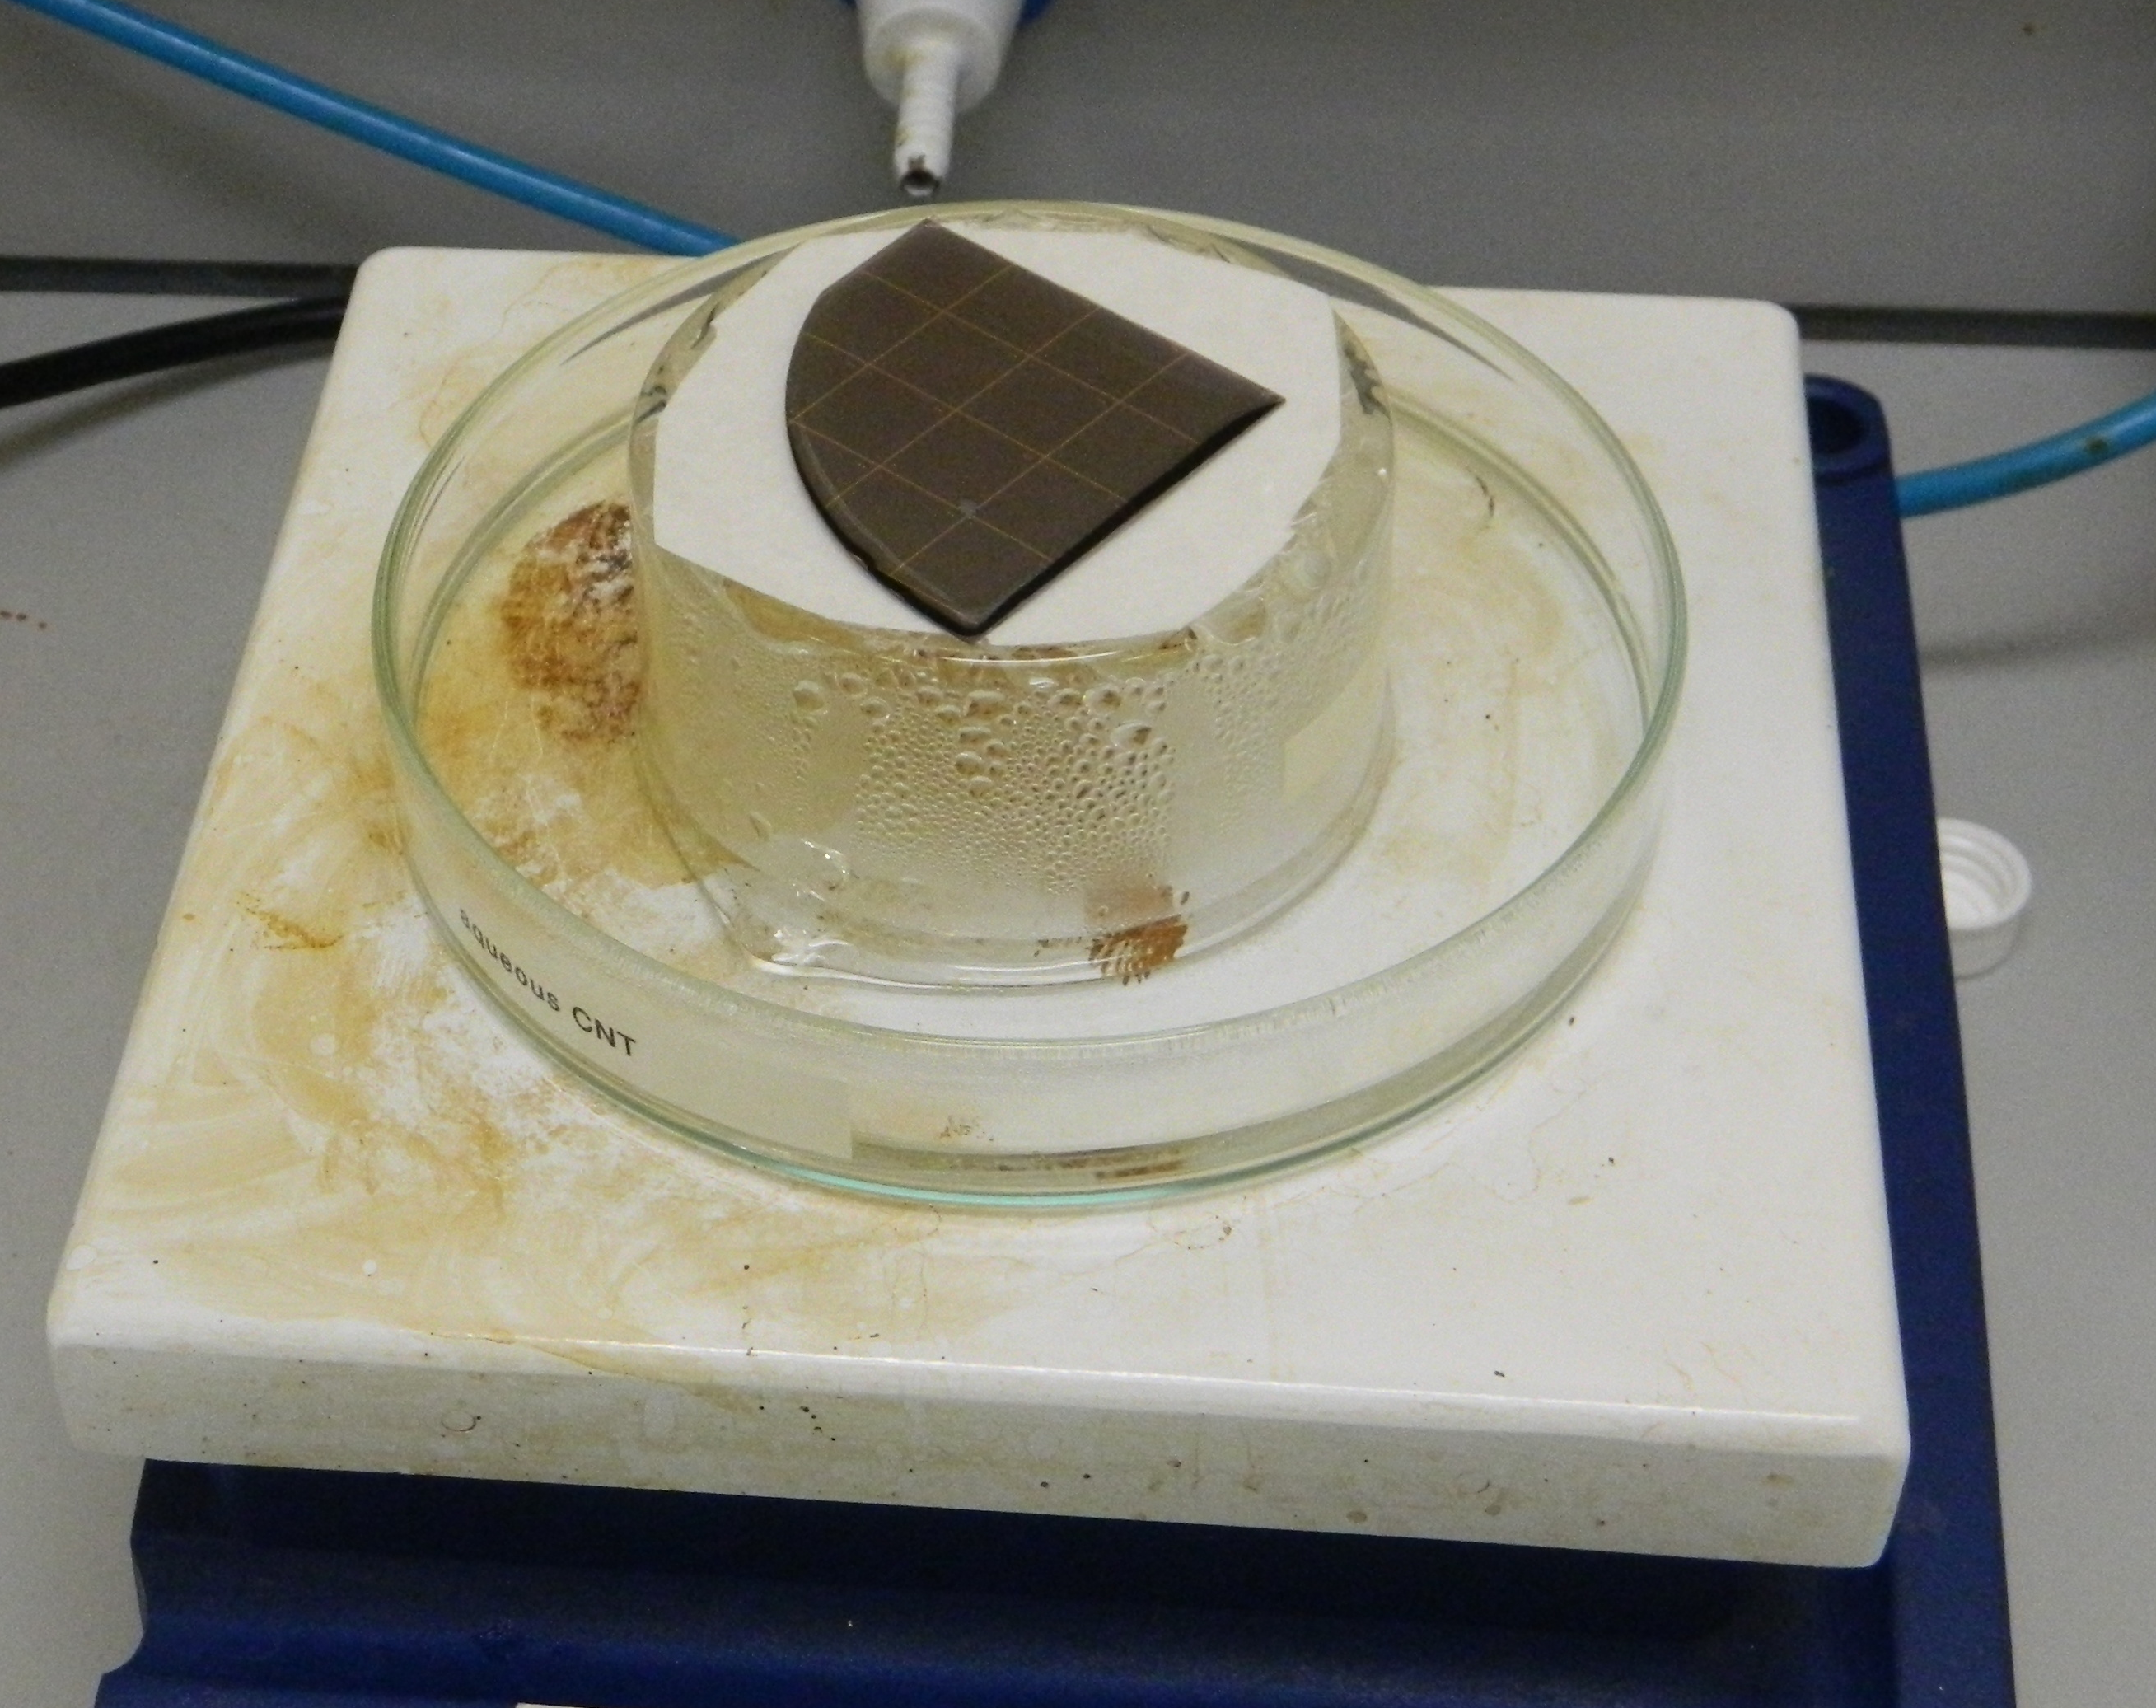
\includegraphics{./figures/ch4/steaming-method-top.png}

}

}

\subcaption{\label{fig-steaming-method-top}Steam method setup without
steam cover}
\end{minipage}%
%
\begin{minipage}[t]{0.05\linewidth}

{\centering 

~

}

\end{minipage}%
%
\begin{minipage}[t]{0.47\linewidth}

{\centering 

\raisebox{-\height}{

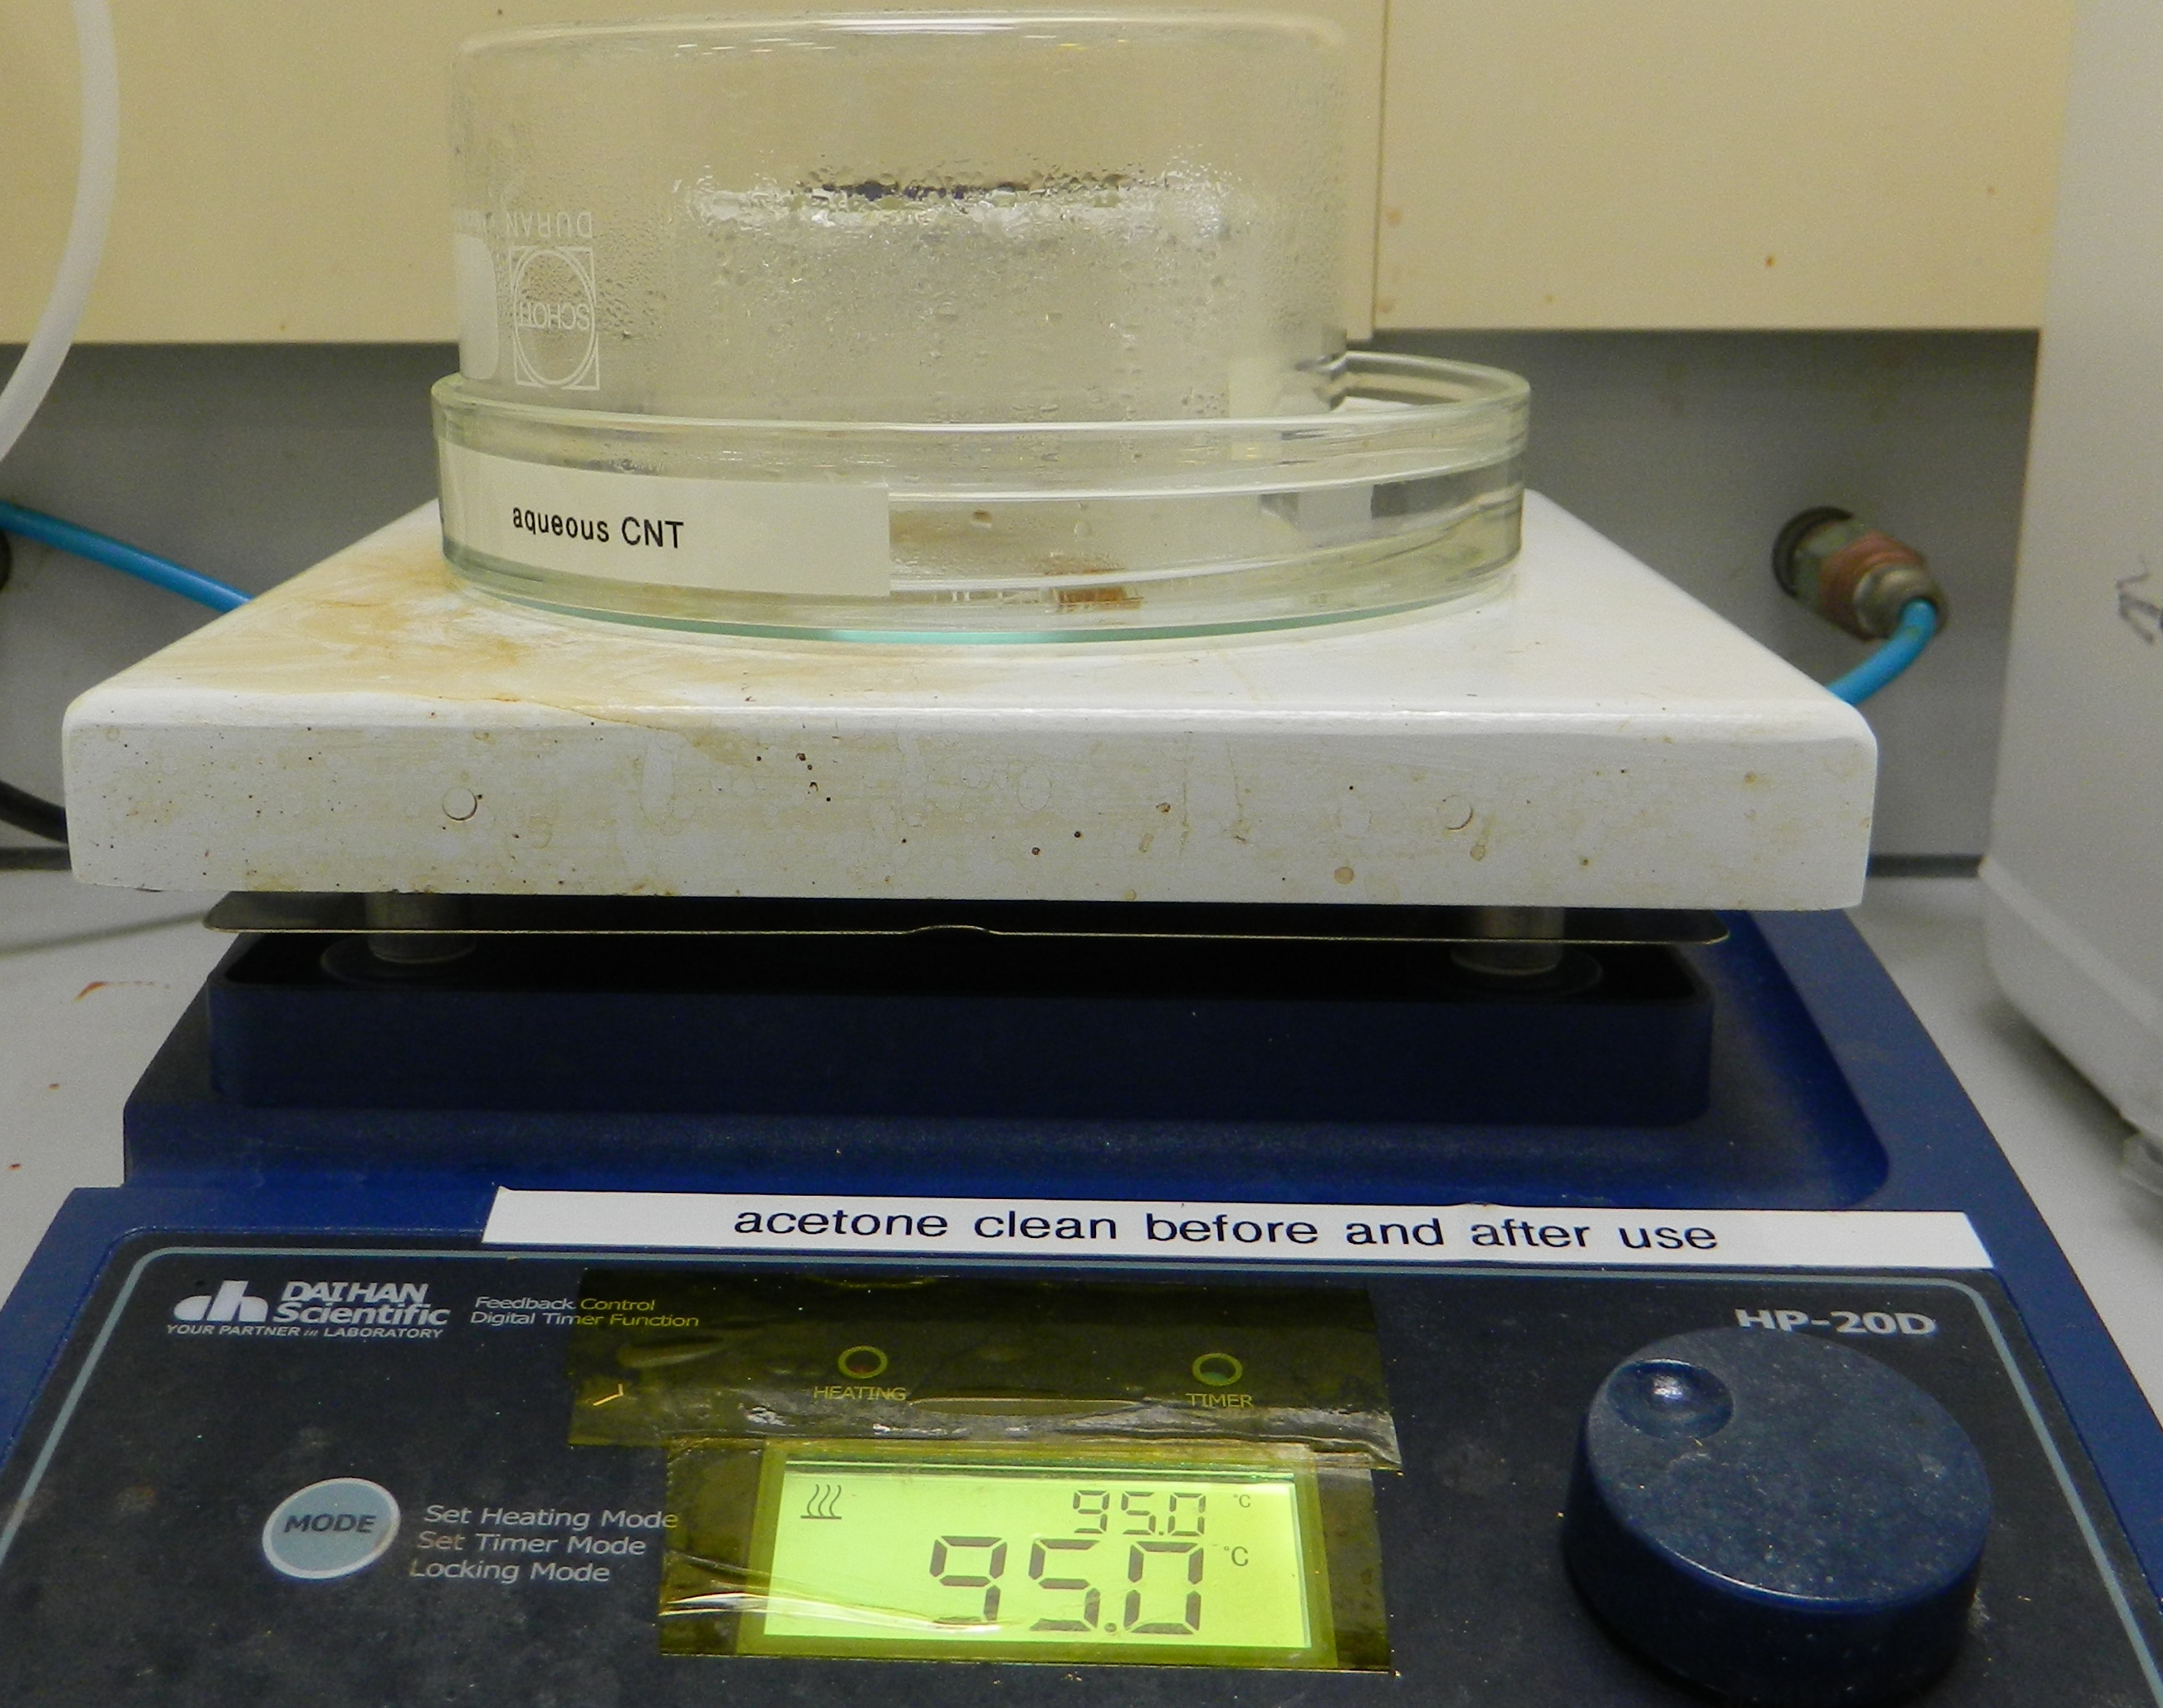
\includegraphics{./figures/ch4/steaming-method-side.png}

}

}

\subcaption{\label{fig-steaming-method-side}Steam method setup with
steam cover}
\end{minipage}%

\caption{\label{fig-steaming-method}Photographs of steam-assisted method
setup (top and side view).}

\end{figure}

2 mL of IsoNanotubes-S 90\% or 99\% solution (NanoIntegris) was decanted
into a small bottle and burst-sonicated once (on then off again) to
break up bundles of CNTs. 75 mL of 95\(^\circ\) C water was then placed
into a glass dish on a hotplate held at 95\(^\circ\) C. After this, the
PLL-functionalised quarter wafer was placed in the centre of an
insulating surface on the same hotplate. The CNT dispersion was
carefully spread across the surface of the wafer without spilling any
over the wafer edges. The wafer on the insulating surface and glass dish
were then left under the same cover for 2 minutes to expose the wafer to
steam from the glass dish. The use of an insulating surface meant that
the wafer and CNT dispersion were not heated from below while exposed to
steam. The steam-assisted deposition setup is shown in
Figure~\ref{fig-steaming-method}.

The CNT dispersion was then rinsed off the wafer with DI water, ethanol,
acetone and IPA, and then the quarter wafer was dried with N\(_2\) gas.
As in the original method, the quarter wafer was then annealed in a
vacuum oven at 150\(^\circ\) C for 1 hour to remove residual surfactant.
This method gave an even spread of CNTs across the quarter wafer
surface, leading to a greater consistency in performance between
devices. Further details can be found in
\textbf{?@sec-cnt-deposition-effects}.

\hypertarget{photolithography-for-carbon-nanotube-and-graphene-field-effect-transistors}{%
\section{Photolithography for Carbon Nanotube and Graphene Field-Effect
Transistors}\label{photolithography-for-carbon-nanotube-and-graphene-field-effect-transistors}}

\begin{figure}

{\centering \includegraphics[width=0.9\textwidth,height=\textheight]{./figures/ch4/photolithography-cycle.png}

}

\caption{\label{fig-qw-photolithography}The photolithographic processes
used for fabrication of both carbon nanotube and graphene devices
(graphene devices were fabricated individually for every step, step \#2
skipped for graphene devices)}

\end{figure}

Photolithography was used to define eight channel regions on each device
and subsequently to define metal contacts for each of these channels. A
schematic demonstrating these photolithography processes on a quarter
wafer is shown in Figure~\ref{fig-qw-photolithography}. Masks for
photolithography were designed in-house using LayoutEditor CAD software
and patterned externally with a UV laser writer.

Thermal evaporation was used when depositing chromium (Cr-plated
tungsten rods, Kurt J. Lesker) and gold (Au wire, 99.99\%, Regal
Castings Ltd.), while electron beam evaporation was used when depositing
titanium (Ti pieces, 99.99\%, Kurt J. Lesker) and metal oxides
(\emph{e.g.} Al\(_2\)O\(_3\) pieces, 99.99\%, Kurt J. Lesker). Metal and
metal oxide deposition was performed using an Angstrom Engineering
Nexdep 200 Vacuum Deposition System. Deposition thickness was controlled
using an Inficon Deposition Controller and electron beam power was
provided by a Telemark TT-6 power supply. For metals, the chamber was
initially evacuated to a pressure \(5 \times 10^{-6}\) mTorr, while for
metal oxides the chamber was initially evacuated to a pressure of
\(1 \times 10^{-5}\) mTorr. After evaporation, the chamber was cooled
and vented with nitrogen.

Carbon nanotube network field-effect transistors were fabricated using
the quarter wafer substrates discussed in
Section~\ref{sec-dep-carbon-nanotubes}.

Graphene field-effect transistors were fabricated using 300 nm
SiO\(_2\)/p-type Si substrates covered with a monolayer of mechanically
transferred CVD graphene (Advanced Chemical Supplier). This substrate
was cleaved into equal-sized square chips before photolithography, with
side length between \(11.6-11.7\) mm, subject to variability in wafer
size. The same cleaving process outlined in
Section~\ref{sec-dep-carbon-nanotubes} was used for cleaving the chips,
but the photoresist was not rinsed off after cleaving. Devices were
exposed to a brief burst of N\(_2\) gas to remove any dust from the
cleaving process from the surface of devices. When not being used in
photolithography, graphene-based devices were stored in a vacuum
desiccator to prevent the quality of the graphene deteriorating with
exposure to air over time. The limited adhesion of graphene to the wafer
meant that photolithographic processing had to be performed particularly
carefully when fabricating graphene devices.

\begin{figure}

\begin{minipage}[t]{0.47\linewidth}

{\centering 

\raisebox{-\height}{

\includegraphics{./figures/ch4/apr-21-dmso-damage.png}

}

}

\subcaption{\label{fig-electrode-dmso-damage}Damage to gold electrode in
channel region after DMSO lift-off}
\end{minipage}%
%
\begin{minipage}[t]{0.05\linewidth}

{\centering 

~

}

\end{minipage}%
%
\begin{minipage}[t]{0.47\linewidth}

{\centering 

\raisebox{-\height}{

\includegraphics{./figures/ch4/may-21-dmso-damage.png}

}

}

\subcaption{\label{fig-graphene-dmso-damage}Damage to graphene (blue
region) after DMSO lift-off}
\end{minipage}%

\caption{\label{fig-dmso-damage}Lift-off with dimethyl sulfoxide
sometimes led to damage to regions where nanomaterials were present.}

\end{figure}

Dimethyl sulfoxide (DMSO) was sometimes used in lift-off processes
instead of acetone between Jul 2021 and Feb 2023 because of its
effectiveness as a photoresist stripping agent. However, it was
abandoned due to some indications it was too aggressive for the devices
being fabricated, as shown in Figure~\ref{fig-dmso-damage} and also as
detailed in \textbf{?@sec-cnt-deposition-effects}. It is possible that
heat from the electrodes deposition sometimes crosslinked residual
photoresist on the nanomaterial, and then during lift-off was removed
aggressively together with any attached nanomaterial by the DMSO.
However, it is also possible that prolonged exposure to DMSO alone was
sufficient to detach nanomaterial from the substrate. Therefore, acetone
was the preferred agent for lift-off despite being a less efficient
stripping agent than DMSO.

From Jul 2023 onwards, after each photolithography step using negative
resist, quarter wafers/chips placed in AZ\(^\circledR\) 326 or SU8
developer for 3 min to ensure complete removal of photoresist residue.
For each step with positive resist, the same procedure was performed but
with a flood exposure with UV light for 1 min before being placed in
developer. The exception to this rule was for devices with an aluminium
oxide layer present. Tetramethylammonium hydroxide (TMAH), the active
ingredient of AZ\(^\circledR\) 326, etches through aluminium oxide and
causes electrical shorts through the dielectric layer
\autocite{Oh2011,Ali2021}. A further discussion showing the results of
this process is given in \textbf{?@sec-photoresist-contamination}.

\hypertarget{sec-align}{%
\subsection{Alignment Markers}\label{sec-align}}

Metal alignment markers were deposited in order to accurately align the
device channels with device electrodes in subsequent photolithography
steps. These alignment markers were asymmetric to indicate the
orientation of the device for subsequent photolithography steps and
electrical characterisation. In later discussion, channel 1 is defined
as the channel placed closest to the large, double square alignment
marker.

For carbon nanotube quarter wafers, alignment markers were deposited
either directly before or after carbon nanotube deposition (see
Section~\ref{sec-dep-carbon-nanotubes} for discussion). For graphene
devices, alignment markers were deposited directly after cleaving using
the protective photoresist layer spincoated prior to cleaving.
AZ\(^\circledR\) 1518 was used for alignment marker photolithography.

For carbon nanotube devices made before Jun 2022, chromium was used as
an adhesive layer for gold, while for all graphene devices and carbon
nanotube devices made after Jun 2022, titanium was used as the adhesive
layer. For chromium/gold depositions, a nominal 10 nm of chromium was
deposited followed by a nominal 100 nm Au layer. For titanium/gold
depositions, a nominal \(10-20\) nm of titanium was deposited followed
by a nominal 50 nm Au layer (for independent measurements of metal layer
thickness, see Section~\ref{sec-electrodes}). Devices were then soaked
in acetone for at least 2 hours for photoresist lift-off, washed in IPA
and dried with nitrogen. The use of titanium gave rise to a cleaner
lift-off and improved gold adhesion. Using a relatively thin gold layer
(50 nm nominal instead of 100 nm) proved to still be clearly visible but
to a cleaner lift-off.

\hypertarget{channel-etching}{%
\subsection{Channel Etching}\label{channel-etching}}

Eight channel features, each 1000 \(\mu\)m in length and 100 \(\mu\)m in
width with a pitch of 1200 \(\mu\)m, were patterned using
AZ\(^\circledR\) 1518 photolithography on each carbon nanotube or
graphene-covered substrate. Unwanted nanomaterial not covered with
photoresist was then etched away with 200 W oxygen plasma at 600 mTorr
using a reactive ion etcher or RIE (Plasmalab\(^\circledR\) 80 Plus,
Oxford Instruments). The etch time was 3 minutes for carbon nanotube
quarter wafers, and 1 minute for graphene chips. The protective
photoresist was then removed by soaking in acetone for at least 5
minutes.

\begin{figure}

\begin{minipage}[t]{0.47\linewidth}

{\centering 

\raisebox{-\height}{

\includegraphics{./figures/ch4/channel-area.png}

}

}

\subcaption{\label{fig-graphene-channel-etch}Graphene channel after
photolithographically defined plasma etch}
\end{minipage}%
%
\begin{minipage}[t]{0.05\linewidth}

{\centering 

~

}

\end{minipage}%
%
\begin{minipage}[t]{0.47\linewidth}

{\centering 

\raisebox{-\height}{

\includegraphics{./figures/ch4/graphene-channel-electrodes.png}

}

}

\subcaption{\label{fig-graphene-channel-electrodes}Graphene channel
after photolithographically defined electrodes deposition and liftoff}
\end{minipage}%

\caption{\label{fig-microscope-graphene-channel}Microscope images of a
graphene channel after plasma etch and electrodes photolithography
steps.}

\end{figure}

\hypertarget{sec-electrodes}{%
\subsection{Electrodes}\label{sec-electrodes}}

\begin{figure}

\begin{minipage}[t]{0.47\linewidth}

{\centering 

\raisebox{-\height}{

\includegraphics{./figures/ch4/dektat_ti_cr_profile_comparison.png}

}

}

\subcaption{\label{fig-dektat-adhesion-layer}Comparison of channel
height profile for the different adhesion layers used (AZ\(^\circledR\)
1518 photolithography used for all profiles)}
\end{minipage}%
%
\begin{minipage}[t]{0.05\linewidth}

{\centering 

~

}

\end{minipage}%
%
\begin{minipage}[t]{0.47\linewidth}

{\centering 

\raisebox{-\height}{

\includegraphics{./figures/ch4/dektat_1518nlof_profile_comparison.png}

}

}

\subcaption{\label{fig-dektat-photoresist-used}Comparison of channel
height profile for the different photoresist types used (titanium
adhesion layer used for all profiles)}
\end{minipage}%

\caption{\label{fig-electrodes-dektat}Dektat height profiles taken
between the source and drain electrodes across a channel from various
quarter wafers with electrodes deposited using different approaches. For
each quarter wafer, the profiles of three different channels are shown,
selected from different locations across the quarter wafer surface.}

\end{figure}

The source and drain electrodes for each channel were patterned using
photolithography with either AZ\(^\circledR\) 1518 photoresist (pre-Mar
2023) or AZ\(^\circledR\) nLOF 2020 photoresist (post-Mar 2023). Before
metal deposition, the developed photoresist pattern was exposed to
O\(_2\) plasma at 50 W for up to 5 s or at 20 W for \(20-25\) s in a
PE-50 plasma cleaner (Plasma Etch, Inc.) to remove residual photoresist
on the developed regions and ensure a clean lift-off. After metal
deposition, wafers/devices were soaked in acetone for at least 2 hours
for photoresist lift-off, washed in IPA and dried with nitrogen.

As with the alignment markers deposition (see Section~\ref{sec-align}),
before Jun 2022 chromium was used for the gold adhesion layer, and after
Jun 2022 titanium was used. Adhesion layers are required to stick metals
such as gold and platinum to silicon dioxide \autocite{Guarnieri2014}. A
20 nm nominal titanium layer instead of 10 nm nominal was found to give
better electrode adhesion, and devices after Feb 2023 were made using
this thicker adhesion layer. Good electronic contact could be made with
electrodes with a nominal gold layer thickness of \(60-100\) nm, and a
Au layer nominally 100 nm thick was most commonly used.

Example height profiles of chromium layer channels and a titanium layer
channels taken using a Veeco Dektat 150 profiler are shown in
Figure~\ref{fig-dektat-adhesion-layer}. AZ\(^\circledR\) 1518
photoresist was used here for photolithographic patterning. A 10 nm
adhesion layer and 100 nm Au layer were used for both depositions to
ensure a consistent comparison. From
Figure~\ref{fig-dektat-adhesion-layer}, we find an measured Cr/Au
electrode height of \(42\pm1\) nm and an measured Ti/Au electrode height
of \(48\pm2\) nm, slightly less than half the respective heights stated
on the Inficon Deposition Controller.

Although using AZ\(^\circledR\) nLOF 2020 photolithography involves more
processing steps, it gave rise to more cleanly-defined electrodes with a
more consistent height profile. Often electrodes deposition using
AZ\(^\circledR\) 1518 photoresist would lead to sharp vertical spikes
along the edge of the electrode. These edge spikes or ``cat ears'' could
partially or fully protrude through thin encapsulation materials such as
SU8 and Al\(_2\)O\(_3\), leading to significant leakage currents from
the electrodes into the FET top gate. This effect is due to the profile
of positive resists being suboptimal for lift-off processes, as
discussed in Appendix~\ref{sec-photolithography}.

The height profiles corresponding to a wafer with electrodes fabricated
using AZ\(^\circledR\) 1518 and to a wafer with electrodes fabricated
using AZ\(^\circledR\) nLOF 2020 are shown in
Figure~\ref{fig-dektat-photoresist-used}. A 20 nm titanium adhesion
layer and 100 nm Au layer were used for both depositions to ensure a
consistent comparison, resulting in a measured electrode height of
\(103\pm2\) nm for both wafers. The wafer which used AZ\(^\circledR\)
nLOF 2020 photoresist clearly has a more consistent electrode height
profile across the wafer surface than the wafer which used
AZ\(^\circledR\) 1518 resist. The measured edge features for the
AZ\(^\circledR\) 1518 resist electrodes vary in size from 20 nm to 450
nm above the bulk electrode surface, whereas the edge features for the
AZ\(^\circledR\) nLOF 2020 resist do not exceed 14 nm in height.

\hypertarget{sec-encapsulation}{%
\subsection{Encapsulation}\label{sec-encapsulation}}

Several different approaches were used for the encapsulation, or contact
protection, of devices. The encapsulation of graphene and
carbon-nanotube transistors for biosensing is essential to improve
transistor characteristics, passivate the electrodes and ensure only the
nanomaterial region is active during biosensing, as discussed in
\textbf{?@sec-biosensor-methods}.

Before encapsulation photolithography the carbon-nanotube network
quarter wafers were cleaved into individual 11 mm \(\times\) 11 mm
chips, using the cleaving process outlined in
Section~\ref{sec-dep-carbon-nanotubes}. Cleaving the devices at this
step simplified mask alignment and ensured consistent thickness across
photoresist encapsulated devices.

Two different photolithography masks were used for encapsulation
photolithography in this work, with different exposed areas of active
nanomaterial. The first mask was used for devices made before Jan 2023,
and was designed to leave a region of 500 \(\mu\)m \(\times\) 10
\(\mu\)m unencapsulated for each channel. The second mask was used
exclusively after Jan 2023, and was designed to leave a region of 200
\(\mu\)m \(\times\) 20 \(\mu\)m unencapsulated for each channel. This
change was made to double the area of carbon nanotubes exposed to
electrolyte while halving the area of SiO\(_2\) dielectric exposed to
electrolyte during aqueous sensing.

\begin{figure}

\begin{minipage}[t]{0.47\linewidth}

{\centering 

\raisebox{-\height}{

\includegraphics{./figures/ch4/encapsulation_old.png}

}

}

\subcaption{\label{fig-encapsulation-old}Encapsulation with
AZ\(^\circledR\) 1518 using pre-2023 mask}
\end{minipage}%
%
\begin{minipage}[t]{0.05\linewidth}

{\centering 

~

}

\end{minipage}%
%
\begin{minipage}[t]{0.47\linewidth}

{\centering 

\raisebox{-\height}{

\includegraphics{./figures/ch4/encapsulation_new.png}

}

}

\subcaption{\label{fig-encapsulation-new}Encapsulation with
AZ\(^\circledR\) 1518 using 2023 mask}
\end{minipage}%

\caption{\label{fig-microscope-encapsulation}Microscope images of carbon
nanotube devices after encapsulation photolithography with hardbaked
AZ\(^\circledR\) 1518.}

\end{figure}

A side-by-side microscope comparison of hardbaked AZ\(^\circledR\) 1518
processed with each mask is given in
Figure~\ref{fig-microscope-encapsulation}, while a Dektat profile
comparison corresponding to Figure~\ref{fig-microscope-encapsulation} is
shown in Figure~\ref{fig-old-new-mask}. The profiles corresponding to
the mask used after Jan 2023 clearly exhibit greater device-to-device
consistency, partly due to the mask requiring a greater level of
accuracy when aligning the encapsulation pattern with the electrode
channel. The larger feature size also means development time has less of
an impact on the quality of the encapsulation opening.

\hypertarget{photoresist-encapsulation}{%
\subsubsection*{Photoresist
encapsulation}\label{photoresist-encapsulation}}
\addcontentsline{toc}{subsubsection}{Photoresist encapsulation}

\begin{figure}

\begin{minipage}[t]{0.47\linewidth}

{\centering 

\raisebox{-\height}{

\includegraphics{./figures/ch4/dektat_oldnewmask_profile_comparison.png}

}

}

\subcaption{\label{fig-old-new-mask}AZ\(^\circledR\) 1518 profiles
comparing pre-2023 mask and mask used from 2023 onwards}
\end{minipage}%
%
\begin{minipage}[t]{0.05\linewidth}

{\centering 

~

}

\end{minipage}%
%
\begin{minipage}[t]{0.47\linewidth}

{\centering 

\raisebox{-\height}{

\includegraphics{./figures/ch4/dektat_SU8_profile_comparison.png}

}

}

\subcaption{\label{fig-SU8-encapsulation}SU-8 2150 profiles comparing
pre-2023 mask and mask used from 2023 onwards}
\end{minipage}%

\caption{\label{fig-dektat-encapsulation}Dektat of carbon nanotube
devices after encapsulation photolithography using hardbaked
AZ\(^\circledR\) 1518 and SU-8 2150, taken from various devices.}

\end{figure}

Two types of photoresist were initially trialled for encapsulation of
carbon nanotube network devices, AZ\(^\circledR\) 1518 and SU8-2150.
Both AZ\(^\circledR\) 1518
\autocite{Thanihaichelvan2018,Thanihaichelvan2019,Shkodra2021} and SU-8
have been previously used for device encapsulation, with SU-8 noted for
being particularly stable and biocompatible
\autocite{Lee2006,Chen2021,Albarghouthi2022}.

Once developed, the photoresist pattern was exposed to O\(_2\) plasma at
50 W for up to 5 s or at 20 W for \(20-25\) s to remove excess
photoresist from the encapsulation opening. Devices were then hardbaked
at 200\(^\circ\)C for 1 hour to fully crosslink the encapsulation layer.
This crosslinking ensured subsequent device exposure to solvent did not
remove the photoresist encapsulation.

The exposed region clear of AZ \(^\circledR\) 1518 resist was
\(6.8 \pm 0.3\) \(\mu\)m in width when using the old, pre-2023 mask,
while the exposed region was \(16.6 \pm 0.4\) \(\mu\)m when using
AZ\(^\circledR\) 1518 with the new mask from 2023, as seen in
Figure~\ref{fig-old-new-mask}. However, the exposed region was reduced
for the SU-8 encapsulation relative to the AZ\(^\circledR\) 1518, with
an width of only 3.6 \(\pm\) 0.5 \(\mu\)m for the pre-2023 mask, as seen
in Figure~\ref{fig-SU8-encapsulation}. Photoresist development using
SU-8 was significantly more time-sensitive than for the AZ\(^\circledR\)
1518. This meant when the development time was increased to create a
wider encapsulation opening, it was difficult to avoid removing large
areas of photoresist across the surface of the encapsulation. This meant
using the new mask from 2023 was especially important for maximising the
exposed channel region of SU-8 devices. Using the new mask from 2023
with the SU-8 resist gave a significantly improved width of 13.8 \(\pm\)
1.0 \(\mu\)m for the exposed region.

A relatively thin SU-8 encapsulation layer could be deposited when
compared to the AZ\(^\circledR\) 1518 encapsulation profile. The
AZ\(^\circledR\) 1518 encapsulation layer had a average height of 1.7
\(\pm\) 0.2 \(\mu\)m, while the SU-8 encapsulation layer had a average
height of 680 \(\pm\) 20 nm. The SU-8 also had much less significant
edge features than the AZ\(^\circledR\) 1518, regardless of the profiles
of the source and drain electrodes.

As noted previously, for both resists the overall profile was more
consistent for the new, 2023 mask from device to device than for the old
pre-2023 mask.

AZ\(^\circledR\) 1518 encapsulation was used for all graphene devices
fabricated.

\hypertarget{dielectric-encapsulation}{%
\subsubsection*{Dielectric
encapsulation}\label{dielectric-encapsulation}}
\addcontentsline{toc}{subsubsection}{Dielectric encapsulation}

\begin{figure}

\begin{minipage}[t]{0.47\linewidth}

{\centering 

\raisebox{-\height}{

\includegraphics{./figures/ch4/Dielectric_Profile_comparison.png}

}

}

\subcaption{\label{fig-dielectric-comparison}Profile comparison of
dielectric materials used for encapsulation}
\end{minipage}%
%
\begin{minipage}[t]{0.05\linewidth}

{\centering 

~

}

\end{minipage}%
%
\begin{minipage}[t]{0.47\linewidth}

{\centering 

\raisebox{-\height}{

\includegraphics{./figures/ch4/al2o3_encapsulation.png}

}

}

\subcaption{\label{fig-al2o3-encapsulation}Microscope image of channel
with aluminium oxide encapsulation}
\end{minipage}%

\caption{\label{fig-dektat-dielectric-layer}Dektat and microscope image
of a device encapsulated with aluminium oxide.}

\end{figure}

Another approach taken was encapsulation of electrode channels with a
dielectric metal oxide/ceramic layer. A electron beam deposition process
was used to deposit a \(100-150\) nm nominal metal oxide layer on
devices patterned with the 2023 mask using AZ\(^\circledR\) nLOF 2020
photoresist. As in Section~\ref{sec-electrodes}, the developed
photoresist pattern was exposed to O\(_2\) plasma at 50 W for up to 5 s
or at 20 W for \(20-25\) s in a PE-50 plasma cleaner (Plasma Etch, Inc.)
before ceramic deposition. Before May 2023, devices were left in
TechniStrip\(^\circledR\) MLO 07 (MicroChemicals) for \(5-10\) min for
lift-off. However, due to concerns over the impact of the constituent
chemical DMSO on the nanomaterial region (see
Figure~\ref{fig-dmso-damage}), the lift-off process was altered from May
2023 onwards. After May 2023, devices were soaked in acetone for at
least 4 hours and sonicated in clean acetone for \(30-60\) s to lift-off
the photoresist, then washed in IPA and dried with nitrogen.

The initial attempt at fabricating a dielectric encapsulation layer used
silicon dioxide as the dielectric. However, silicon dioxide adheres
poorly to gold without an metallic adhesive layer present, as shown in
Figure~\ref{fig-dielectric-comparison}. Aluminium oxide was chosen as an
alternative as it sticks well to bulk electrode materials, is heat and
chemical resistant, has a relatively high dielectric constant and is
bio-compatible \autocite{Guarnieri2014,Albarghouthi2022,Kolodzey2000}.
Figure~\ref{fig-dektat-dielectric-layer} shows the aluminium oxide
successfully adhered to the electrodes and had a clean profile
comparable to that of the SU-8 encapsulation layer after lift-off. As
noted earlier, aluminium oxide should not be subsequently exposed to its
etchant TMAH.

\hypertarget{sec-afm-characterisation}{%
\section{Characterisation via Atomic Force
Microscopy}\label{sec-afm-characterisation}}

Atomic force microscopy in this thesis was taken using a Nanosurf
NaioAFM in dynamic force mode (also known as tapping mode, oscillating
mode, acoustic AC mode or intermittent-contact mode). An ACLA probe
(AppNano) was used with a tip diameter of 12 nm, height of \(14-16\)
\(\mu\)m and a nominal cantilever spring constant of 58 N/m. All atomic
force microscopy was performed with the Nanosurf NaioAFM on a stablising
table under a Faraday cage to minimise mechanical and electromagnetic
interference. A 256 \(\times\) 256 pixel resolution was typically used.
Imaging was performed in air at room temperature.

Atomic force microscope (AFM) images could not be taken from the small
exposed channel region on the encapsulated devices, so were instead
taken on a representative carbon nanotube or graphene film sample
fabricated on the same wafer as the device being tested. Moisture
adversely affected the AFM imaging process. Therefore, films
functionalised with biological materials were washed with DI water and
gently dried with N\(_2\) before atomic force microscope images were
taken.

The open source data analysis software Gwyddion (version 2.59) was used
to analyse AFM images. This included levelling the background with the
polynomial background removal function, removing scarring and zeroing
the z-scale.

\hypertarget{sec-fluorescence-characterisation}{%
\section{Characterisation via Fluorescence
Microscopy}\label{sec-fluorescence-characterisation}}

Fluorescence microscopy was taken using an Olympus BX63 fluorescence
microscope controlled using cellSens imaging software. Microscope
objectives used were all Olympus UPLSAPO/UPlanSApo, apochromat
objectives which compensate for spherical and chromatic aberrations.
Objectives had infinite aperture and a field number of 26.5. Filter
cubes used included the Olympus FITC filter (excitation wavelength
range: \(467-498\) nm, emission wavelength range: \(513-556\) nm), Texas
Red (excitation wavelength range: \(542-582\) nm, emission wavelength
range: \(604-644\) nm) and GFP (excitation wavelength range: \(604-644\)
nm, emission wavelength range: \(502-538\) nm). The ISO was kept at the
lowest available setting, ISO200. All microscopy was performed in
darkness with the screen turned away from the microscope. To ensure
photobleaching did not adversely affect imaging, images were taken soon
after initial exposure to fluorescence and taking repeated photos of the
same region was avoided. Various useful and thourough introductions to
fluorescence microscopy can be found online \autocite{Nikon,Zeiss}.

\hypertarget{sec-electrical-characterisation}{%
\section{Electrical
Characterisation}\label{sec-electrical-characterisation}}

\begin{figure}

{\centering \includegraphics[width=0.9\textwidth,height=\textheight]{./figures/ch4/liquid-gate-schematic.png}

}

\caption{\label{fig-liquid-gate-schematic}Liquid-gated device schematic
showing electrical connections to the three source measure units.
V\(_{\mathrm{ds}}\) is applied between the source SMU (SMU 1) and the
drain SMU (SMU 2), while V\(_{\mathrm{lg}}\) is applied between the gate
SMU (SMU 3) and the drain SMU. The drain SMU is held at 0 V or connected
to a ground plane. Drain current I\(_{\mathrm{d}}\) is measured at the
drain SMU, and gate leakage current I\(_{\mathrm{g}}\) is measured at
the gate SMU.}

\end{figure}

Both back-gated and liquid-gated measurements were taken of carbon
nanotube and graphene devices. Liquid-gated measurements were taken
using the configuration shown in Figure~\ref{fig-liquid-gate-schematic}.
Back-gated measurements were taken with a copper plane placed underneath
the Si/SiO\(_2\) wafer and connected to SMU 3 instead of the reference
electrode.

All measurement setups used had the same basic configuration, with two
source measure units (SMUs) attached to the source and gate. Voltage
from the source and gate SMUs was either kept constant or varied, with
only one SMU varied at a time. Three different measurement setups were
used for taking these measurements, the Keysight (Agilent/HP) 4156C
Semiconductor Parameter Analyser, the Keysight B1500A Semiconductor
Device Analyser, and a National Instruments NI-PXIe modular measurement
system with a 8 GB PXIe-8821 controller and two NI-4138 source measure
units. For measurements with the Keysight instruments, a third, drain
SMU was attached and kept at a constant 0 V (as shown in
Figure~\ref{fig-liquid-gate-schematic}).

\begin{figure}

\begin{minipage}[t]{0.47\linewidth}

{\centering 

\raisebox{-\height}{

\includegraphics{./figures/ch4/PDMS_dirty.png}

}

}

\subcaption{\label{fig-PDMS_dirty}PDMS surface before sonication in IPA
for 10 min}
\end{minipage}%
%
\begin{minipage}[t]{0.05\linewidth}

{\centering 

~

}

\end{minipage}%
%
\begin{minipage}[t]{0.47\linewidth}

{\centering 

\raisebox{-\height}{

\includegraphics{./figures/ch4/PDMS_clean.png}

}

}

\subcaption{\label{fig-PDMS_clean}PDMS surface after sonication in IPA
for 10 min}
\end{minipage}%

\caption{\label{fig-PDMS-clean}Polydimethylsiloxane (PDMS) surface
before and after isopropanol (IPA) sonication for 10 minutes.}

\end{figure}

When using the Keysight 4156C Semiconductor Parameter Analyser or
Keysight B1500A Semiconductor Device Analyser for liquid-gated
measurements, a Rucker and Kolls with micromanipulators was used to
contact the devices; when using the National Instruments NI-PXIe for
liquid-gated measurements, a custom-made chip carrier with
spring-loaded, pointed-tip, gold-coated pogo pins was used. Ag/AgCl
standard electrodes were used as the liquid-gate electrode. The
electrode was submerged in 80 \(\mu\)L of PBS buffer in a
polydimethylsiloxane (PDMS) well with outer dimensions of 12 mm
\(\times\) 6 mm \(\times\) 6 mm. This PDMS well was sonicated in
isopropanol for 10 min and thoroughly N\(_2\) dried before use. The
microscope images seen in Figure~\ref{fig-PDMS-clean} show the PDMS
surface before and after this cleaning step. The end of Ag/AgCl standard
electrode to be submerged should be rinsed in DI water and left to sit
in DI water for 15 minutes before characterisation is performed.

The Keysight 4156C Semiconductor Parameter Analyser and Keysight B1500A
Semiconductor Device Analyser were also used for back-gated measurements
of devices within the vapour delivery system device chamber. This
chamber acted as a Faraday cage for another custom-made chip carrier
with spring-loaded gold-coated pogo pins, able to contact four channel
electrode pairs at once. The silicon back of the device was pressed by
the pins against a copper block, connected to the gate SMU.

Custom programs for National Instruments LabView 2017 were used for
measurements from the Keysight 4156C Semiconductor Parameter Analyser
and the National Instruments NI-PXIe. Keysight EasyEXPERT software was
used for characterisation with the Keysight B1500A Semiconductor Device
Analyser.

Liquid-gated transfer characteristics of carbon nanotube FETs were
measured at V\(_{\mathrm{ds}}\) = 100 mV and liquid-gated transfer
characteristics of graphene FETs were measured at V\(_{\mathrm{ds}}\) =
1 V, where V\(_{\mathrm{lg}}\) was swept between -0.5 V and 1 V in both
the forward and reverse direction with a step size of either 10 or 20
mV. Backgated transfer characteristics of carbon nanotube FETs were
either measured at V\(_{\mathrm{ds}}\) = 100 mV or V\(_{\mathrm{ds}}\) =
1 V, where V\(_{\mathrm{bg}}\) was swept between -5 V and 5 V or -10 V
and 10 V in the forward and reverse directions with a step size of 50 mV
or 100 mV.

\hypertarget{sensing-measurements}{%
\subsection{Sensing Measurements}\label{sensing-measurements}}

A liquid-gated setup was used for aqueous-phase sensing and a back-gated
setup in the vapour delivery system was used for vapour-phase sensing,
as described above.

Sensing measurements were performed with constant source-drain and gate
voltages. The gate voltage used was chosen by locating the subthreshold
region of the device transfer characteristics and choosing a voltage
that fell within this region, usually V\(_{\mathrm{g}}\) = 0 V.

Using the NI-PXIe with the PXIe-2737 module, eight-channel multiplexed
current measurements could be taken in rapid succession. An integration
time of 200 or 400 ms was used for sampling with each channel, with the
actual sampling rate set by the NI-PXIe. In practice this meant a
sampling rate of 1.81 s (for 200 ms integration time) or 3.41 s (for 400
ms integration time) for any given channel. A 200 ms integration time
meant the time between samples from successive channels varied between
\(220 ms-230\) ms, while a 400 ms integration time meant the time
between samples was consistently 426 ms. The Keysight equipment used a
constant 1 s sampling interval.

\hypertarget{aqueous-sensing}{%
\subsubsection*{Aqueous Sensing}\label{aqueous-sensing}}
\addcontentsline{toc}{subsubsection}{Aqueous Sensing}

Before the sensing process, 200 \(\mu\)L of PBS was added to the PDMS
well and 100-120 \(\mu\)L of PBS was removed. This initial step was
performed to wet the sides of the PDMS well, and check that the
attachment of the PDMS well to the device would not unseal when larger
volumes of PBS were added during sensing. Before any sensing
measurement, a transfer characteristic curve was taken of the
liquid-gated device. From Feb 2022 onwards, a 1800 s control series was
performed as part of each sensing experiment to test for unwanted
responses to PBS and to allow baseline drift to settle. 20 \(\mu\)L
additions of PBS were added to the PDMS well at 100 s, 200 s and 300 s,
and 20 \(\mu\)L of PBS were removed from the PDMS well at 400 s, 500 s
and 600 s. Immediately after the control series, a sensing sequence was
performed as part of the same continuous measurement set. Most commonly,
this would consist of a final PBS addition at 2100 s, then analyte
additions every 300 s after that. The experimental series was set to
finish at 4000 s. The exact timings, analyte concentrations and gate
voltage used in a given sensing sequence are discussed alongside the
relevant experimental results.

\hypertarget{vapour-sensing}{%
\subsubsection*{Vapour Sensing}\label{vapour-sensing}}
\addcontentsline{toc}{subsubsection}{Vapour Sensing}

A variety of vapour sensing sequences were used in this work, which are
discussed in \textbf{?@sec-vapour-sensing-biosensors} in detail.

\hypertarget{summary}{%
\section{Summary}\label{summary}}

A variety of approaches were trialled when depositing a carbon nanotube
network for the fabrication of transistor devices, and the resultant
morphology of these networks are discussed in the next chapter. Standard
photolithographic methods were used to successfully fabricate carbon
nanotube and graphene field effect transistor devices. A range of
photolithography types and electrode/encapsulation materials were
trialled to find the optimal device composition for sensing, also
discussed in the next chapter. Atomic force microscopy, fluorescence
microscopy and a variety of electrical measurement setups were used to
characterise the devices.

\bookmarksetup{startatroot}

\hypertarget{characteristics-of-pristine-carbon-nanotube-graphene-field-effect-transistors}{%
\chapter{Characteristics of Pristine Carbon Nanotube \& Graphene Field
Effect
Transistors}\label{characteristics-of-pristine-carbon-nanotube-graphene-field-effect-transistors}}

\begin{verbatim}
158862
\end{verbatim}

\hypertarget{sec-pristine-morphology}{%
\section{Carbon Nanotube Network
Morphology}\label{sec-pristine-morphology}}

Figure~\ref{fig-afm-morphology} shows a side-by-side comparison of the
surface morphology of carbon nanotube films fabricated using the methods
described in Section~\ref{sec-dep-carbon-nanotubes}. These images were
collected using an atomic force microscope and processed in the manner
described in Section~\ref{sec-afm-characterisation}. They each show
bundles of carbon nanotubes with a range of diameters and lengths, with
each bundle containing one or multiple nanotubes. As discussed in
previous works using solvent-based deposition techniques for depositing
carbon nanotubes, multi-tube bundles form due to strong mutual
attraction between nanotubes
\autocite{Zheng2017,Thanihaichelvan2018,Thanihaichelvan2019,Nguyen2021}.
However, when surfactants are present, they adsorb onto the carbon
nanotubes and form a highly repulsive structure able to overcome the
strong attraction between nanotubes. This repulsion then keeps the
individual carbon nanotubes isolated
\autocite{Wenseleers2004,Shimizu2013}. The diameter range provided by
the supplier for the individual carbon nanotubes used is \(1.2-1.7\) nm,
while the length range is \(0.3-5.0\) \(\mu\)m (Nanointegris).

\begin{figure}

\begin{minipage}[t]{0.47\linewidth}

{\centering 

\raisebox{-\height}{

\includegraphics{./figures/ch5/Ned_NTQ24_20220125_00235.png}

}

}

\subcaption{\label{fig-bundled-network}Solvent-based deposition}
\end{minipage}%
%
\begin{minipage}[t]{0.05\linewidth}

{\centering 

~

}

\end{minipage}%
%
\begin{minipage}[t]{0.47\linewidth}

{\centering 

\raisebox{-\height}{

\includegraphics{./figures/ch5/Ned_NTQ24_20220125_00235_histogram_guess.png}

}

}

\subcaption{\label{fig-bundled-network-histogram}Solvent based
deposition histogram}
\end{minipage}%
\newline
\begin{minipage}[t]{0.47\linewidth}

{\centering 

\raisebox{-\height}{

\includegraphics{./figures/ch5/Ned_NTQ8C7_w4_pristine_00084_20210428(2).png}

}

}

\subcaption{\label{fig-dropcast-network}Dropcast surfactant-based
deposition}
\end{minipage}%
%
\begin{minipage}[t]{0.05\linewidth}

{\centering 

~

}

\end{minipage}%
%
\begin{minipage}[t]{0.47\linewidth}

{\centering 

\raisebox{-\height}{

\includegraphics{./figures/ch5/Ned_NTQ8C7_w4_pristine_00084_20210428(2)_histogram_guess.png}

}

}

\subcaption{\label{fig-dropcast-network-histogram}Dropcast
surfactant-based deposition histogram}
\end{minipage}%
\newline
\begin{minipage}[t]{0.47\linewidth}

{\centering 

\raisebox{-\height}{

\includegraphics{./figures/ch5/Ned_NGQ14D2_W4_pristine_20220713_00567.png}

}

}

\subcaption{\label{fig-steaming-network}Steam-assisted dropcast
surfactant-based deposition}
\end{minipage}%
%
\begin{minipage}[t]{0.05\linewidth}

{\centering 

~

}

\end{minipage}%
%
\begin{minipage}[t]{0.47\linewidth}

{\centering 

\raisebox{-\height}{

\includegraphics{./figures/ch5/Ned_NGQ14D2_W4_pristine_20220713_00567_histogram_guess.png}

}

}

\subcaption{\label{fig-steaming-network-histogram}Steam-assisted
dropcast surfactant-based deposition}
\end{minipage}%

\caption{\label{fig-afm-morphology}2.5 \(\mu\)m \(\times\) 2.5 \(\mu\)m
atomic force microscope (AFM) images of carbon nanotube films deposited
using various methods, shown side-by-side with surface profile
histograms extracted from the AFM profile. Each histogram is shown
alongside a linear combination of normal distributions \#1 and \#2,
corresponding to the silicon and carbon nanotube distribution
respectively. The counts remaining after \#1 and \#2 have been
subtracted from the AFM histogram are shown in blue.}

\end{figure}

The diameter range of deposited single-walled carbon nanotubes can be
modelled via a normal or Gaussian distribution
\autocite{LeMieux2008,Liu2013,Thanihaichelvan2018,Vobornik2023}.
However, when we extract and bin the height profiles from the 2.5
\(\mu\)m \(\times\) 2.5 \(\mu\)m AFM images, plotted in black in
Figure~\ref{fig-afm-morphology}, the histograms do not follow a normal
distribution. The reason for this result is that the carbon nanotubes do
not lie perfectly level on a perfectly level silicon oxide substrate -
the atomic force microscope histogram would only be a single normal
distribution in this ideal case. In practice, the SiO\(_2\) substrate
and carbon nanotube surface both have a degree of roughness, which may
in part be due to the presence of atmospheric contaminants. In the case
of the surfactant-deposited networks, residual surfactant may also
contribute to surface roughness \autocite{Vobornik2023}. Furthermore,
nanotubes overlap and cross over each other, creating junctions with the
combined height of the overlapping nanotubes.

It has been demonstrated that the surface roughness of a bare SiO\(_2\)
substrate can also be modelled with a normal distribution. This normal
distribution can be set as the reference or zero point for other height
measurements \autocite{Velicky2015}. As both the carbon nanotube and
silicon dioxide background heights can each be modelled using a normal
distribution, we make an initial assumption that a linear combination of
normal distributions can be used to model the AFM histograms in
Figure~\ref{fig-afm-morphology}. Using the process discussed in
Section~\ref{sec-histogram-analysis}, we approximate the normal
distributions corresponding to the silicon oxide substrate and carbon
nanotube network, shown in Figure~\ref{fig-afm-morphology} as green and
red curves respectively. The silicon oxide peak appears to fit more
closely to the distribution with smaller carbon nanotube heights, which
could be due to measurement of the silicon background being improved
when feature height is smaller. We notice that the distribution for the
carbon nanotube bundles drops to approximately zero before reaching 0
nm, which is physically appropriate.

\begin{figure}

\begin{minipage}[t]{0.47\linewidth}

{\centering 

\raisebox{-\height}{

\includegraphics{./figures/ch5/Ned_NTQ24_20220125_00235_half_histogram_fit.png}

}

}

\subcaption{\label{fig-bundled-network-remainder}Solvent based
deposition histogram}
\end{minipage}%
%
\begin{minipage}[t]{0.05\linewidth}

{\centering 

~

}

\end{minipage}%
%
\begin{minipage}[t]{0.47\linewidth}

{\centering 

\raisebox{-\height}{

\includegraphics{./figures/ch5/Ned_NTQ8C7_w4_pristine_00084_20210428(2)_half_histogram_fit.png}

}

}

\subcaption{\label{fig-dropcast-network-remainder}Dropcast
surfactant-based deposition histogram}
\end{minipage}%
\newline
\begin{minipage}[t]{0.26\linewidth}

{\centering 

~

}

\end{minipage}%
%
\begin{minipage}[t]{0.47\linewidth}

{\centering 

\raisebox{-\height}{

\includegraphics{./figures/ch5/Ned_NGQ14D2_W4_pristine_20220713_00567_half_histogram_fit.png}

}

}

\subcaption{\label{fig-steaming-network-remainder}Steam-assisted
dropcast surfactant-based deposition}
\end{minipage}%
%
\begin{minipage}[t]{0.26\linewidth}

{\centering 

~

}

\end{minipage}%

\caption{\label{fig-remaining-histogram}The counts which remain after
\#1 and \#2 have been subtracted from the AFM histogram are shown in
black. The counts have been overlaid with half a Gaussian distribution,
manually fitted.}

\end{figure}

By subtracting the modelled silicon and carbon nanotube normal
distributions from the AFM histogram, we find a remaining distribution
spread roughly between 0 nm and the mean of the carbon nanotube bundle
distribution. Interestingly, the peak of the carbon nanotube
distribution occurs at a height approximately 2.5\(\times\) the height
corresponding to the peak of the remaining distribution. It is also
apparent that the remaining distribution consistently follows a normal
distribution after a sharp rise to maximum, as shown in
Figure~\ref{fig-remaining-histogram}. This distribution appears to
correspond to surface roughness due to the presence of contaminants, or
possibly to broken pieces of individual nanotubes with various lengths.
Contaminants could be residual surfactant or other atmospheric
contamination resistant to acetone and isopropanol rinsing. Such
contamination may or may not have implications for biosensing
suitability, but surfactant contamination could certainly have negative
effects on biological elements sensitive to surfactant. The area of this
central peak may be useful for determining the extent of contamination
on a carbon nanotube film, discussed further in
\textbf{?@sec-contamination}.

If we model carbon nanotube bundles as cylinders, and we assume the
component nanotubes follow 2D packing and are of equal diameter, we can
give an estimate the mean bundle size for each deposition type in terms
of number of nanotubes \emph{n}
\autocite{Graham1998,Thanihaichelvan2018,Specht2023}.

\hypertarget{tbl-circle-packing}{}
\begin{longtable}[]{@{}
  >{\raggedright\arraybackslash}p{(\columnwidth - 16\tabcolsep) * \real{0.1053}}
  >{\raggedright\arraybackslash}p{(\columnwidth - 16\tabcolsep) * \real{0.1228}}
  >{\raggedright\arraybackslash}p{(\columnwidth - 16\tabcolsep) * \real{0.0965}}
  >{\raggedright\arraybackslash}p{(\columnwidth - 16\tabcolsep) * \real{0.0965}}
  >{\raggedright\arraybackslash}p{(\columnwidth - 16\tabcolsep) * \real{0.1228}}
  >{\raggedright\arraybackslash}p{(\columnwidth - 16\tabcolsep) * \real{0.1228}}
  >{\raggedright\arraybackslash}p{(\columnwidth - 16\tabcolsep) * \real{0.1228}}
  >{\raggedright\arraybackslash}p{(\columnwidth - 16\tabcolsep) * \real{0.1228}}
  >{\raggedright\arraybackslash}p{(\columnwidth - 16\tabcolsep) * \real{0.0877}}@{}}
\caption{\label{tbl-circle-packing}The first eight optimised ratios of
2D packed circle diameter to encompassing circle diameter, given to 3
s.f. (encompassing circle diameter = \(d\), number of packed circles =
\(n\), approximate packed circle diameter = \(d_n\)).\\
}\tabularnewline
\toprule()
\endhead
\(n\) & \text{2} & \text{3} & \text{4} & \text{5} & \text{6} & \text{7}
& \text{8} & \text{9} \\
\(d\)/\(d_n\) & \text{2.00} & 2.15 & 2.41 & \text{2.70} & \text{3.00} &
\text{3.00} & \text{3.30} & 3.61 \\
\bottomrule()
\end{longtable}

Table~\ref{tbl-circle-packing} shows the relationship between the
diameter of a bundle and the constituent diameters of up to nine 2D
packed carbon nanotubes within that bundle. Assuming an average carbon
nanotube diameter of 1.45 nm, we can use the \(d\)/\(d_n\) packing
ratios to obtain an estimate of the number of nanotubes in the mean
bundle size for each deposition \autocite{Specht2023}. We can also give
an approximate range which this estimate falls within using the provided
range of individual carbon nanotube diameters (\(1.2-1.7\) nm) and the
95\% confidence interval of the mean bundle size (\(2\sigma\)). These
estimates are shown in Table~\ref{tbl-histogram-parameters}. Also shown
is an estimate of the ratio of single- to multi-tube bundles for each
deposition, found by comparing the proportion of each carbon nanotube
curve below and above 2.9 nm, the minimum multi-tube bundle size for
1.45 nm diameter nanotubes. It should be noted that the force of the
atomic force microscope tip may cause some degree of nanotube bundle
compression, leading to a systematic underestimate of nanotube height
\autocite{Vobornik2023}. The relative proportion of multi-tube bundles
shown in Table~\ref{tbl-histogram-parameters} should therefore be
treated as a lower-limit estimate of the true proportion.

\hypertarget{tbl-histogram-parameters}{}
\begin{table}
\caption{\label{tbl-histogram-parameters}The mean of histogram distributions for carbon nanotube films deposited
using various methods, alongside estimates for the number of nanotubes
present per bundle (within a 95\% confidence interval) and the
proportion of multi-tubed bundles present across the network. The value
in brackets corresponds to an estimate for the number of nanotubes
present in the mean bundle size. }\tabularnewline

\centering
\begin{tabular}{>{\raggedright\arraybackslash}p{2cm}ccccc}
\toprule
\multicolumn{1}{c}{\textbf{ }} & \multicolumn{3}{c}{\textbf{Distribution Mean (nm)}} & \multicolumn{2}{c}{\textbf{Bundle Attributes}} \\
\cmidrule(l{3pt}r{3pt}){2-4} \cmidrule(l{3pt}r{3pt}){5-6}
 & Silicon & Bundles & Contaminant & Tubes/Bundle & \% Multi-Tube\\
\midrule
Solvent deposited & 0.0 ± 1.4 & 8.8 ± 4.0 & 3.6 ± 3.8 & 1–162 (28) & > 95\%\\
 &  &  &  &  \vphantom{1} & \\
Surfactant deposited & 0.0 ± 0.6 & 5.1 ± 1.4 & 2.0 ± 1.5 & 1–34 (8) & > 94\%\\
 &  &  &  &  & \\
Surfactant deposited with steam & 0.0 ± 0.5 & 3.2 ± 1.1 & 1.2 ± 0.9 & 1–15 (3) & > 60\%\\
\bottomrule
\end{tabular}
\end{table}

When surfactant is used in the deposition process, both the carbon
nanotube bundle diameter mean and standard deviation are small compared
to the mean and standard deviation of solvent deposited films. However,
despite the presence of surfactant, it is apparent both from
Figure~\ref{fig-afm-morphology} and Table~\ref{tbl-histogram-parameters}
that not all surfactant-dispersed carbon nanotubes are deposited
individually. Bundling may occur during the process of deposition onto
the substrate, which could disrupt the repulsive forces from the
surfactant coating and allow attractive forces to temporarily dominate.

It is possible that the bundling of surfactant-dispersed carbon
nanotubes is a consequence of dynamics introduced by the coffee-ring
effect \autocite{Deegan1997,VanGaalen2021}. The coffee-ring effect
refers to a build-up of dispersed solid forming around the edges of a
dispersion evaporating on a surface. This process occurs due to the
dispersion edges being fixed by surface forces, leading to capillary
flow outwards to replace liquid evaporating at the edges, bringing solid
material along with it. The presence of vapour is known to disrupt this
capillary effect \autocite{Bishop2020}.

\hypertarget{sec-pristine-electrical-characterisation}{%
\section{Electrical Characteristics of Pristine
Devices}\label{sec-pristine-electrical-characterisation}}

\hypertarget{carbon-nanotube-network-devices}{%
\subsection{Carbon Nanotube Network
Devices}\label{carbon-nanotube-network-devices}}

\begin{figure}

\begin{minipage}[t]{0.49\linewidth}

{\centering 

\raisebox{-\height}{

\includegraphics{./figures/ch5/NTQ22C2_solvent_backgate.png}

}

}

\subcaption{\label{fig-solvent-tx-bg}Solvent-based deposition,
back-gated}
\end{minipage}%
%
\begin{minipage}[t]{0.02\linewidth}

{\centering 

~

}

\end{minipage}%
%
\begin{minipage}[t]{0.49\linewidth}

{\centering 

\raisebox{-\height}{

\includegraphics{./figures/ch5/NTQ24C8_pristine_TXLG01_220211_solvent_gate.png}

}

}

\subcaption{\label{fig-solvent-tx-lg}Solvent-based deposition,
liquid-gated}
\end{minipage}%
\newline
\begin{minipage}[t]{0.49\linewidth}

{\centering 

\raisebox{-\height}{

\includegraphics{./figures/ch5/Q5C10_nosteam_backgate.png}

}

}

\subcaption{\label{fig-surf-tx-bg}Dropcast surfactant-based deposition,
back-gated}
\end{minipage}%
%
\begin{minipage}[t]{0.02\linewidth}

{\centering 

~

}

\end{minipage}%
%
\begin{minipage}[t]{0.49\linewidth}

{\centering 

\raisebox{-\height}{

\includegraphics{./figures/ch5/NTQ5C3_pristine_TXLG01_210602_nosteam_gate.png}

}

}

\subcaption{\label{fig-surf-tx-lg}Dropcast surfactant-based deposition,
liquid-gated}
\end{minipage}%
\newline
\begin{minipage}[t]{0.49\linewidth}

{\centering 

\raisebox{-\height}{

\includegraphics{./figures/ch5/Q18C6_steam_backgate.png}

}

}

\subcaption{\label{fig-steam-tx-bg}Steam-assisted dropcast
surfactant-based deposition, back-gated}
\end{minipage}%
%
\begin{minipage}[t]{0.02\linewidth}

{\centering 

~

}

\end{minipage}%
%
\begin{minipage}[t]{0.49\linewidth}

{\centering 

\raisebox{-\height}{

\includegraphics{./figures/ch5/NTQ31C6_pristine_TXLG01_230330_steam_gate.png}

}

}

\subcaption{\label{fig-steam-tx-lg}Steam-assisted dropcast
surfactant-based deposition, liquid-gated}
\end{minipage}%

\caption{\label{fig-pristine-cnt-characteristics}Transfer
characteristics of AZ\(^\circledR\) 1518 encapsulated field-effect
transistors with carbon nanotube network channels deposited using
various methods. 1XPBS was used as the buffer for the liquid-gated
measurements here. The source-drain voltage used for all sweeps was
\(V_{ds} = 100 \textrm{mV}\). A step size of 20 mV was used for the
liquid-gated sweeps, while a step size of 100 mV was used for the
backgated sweeps. Each pair of sweeps was taken from a separate device.
Devices with a 100 nm SiO\(_2\) layer were used for backgated
measurements, and devices with a 300 nm SiO\(_2\) layer were used for
liquid gated measurements.}

\end{figure}

Each carbon nanotube device fabricated was electrically characterised as
described in Section~\ref{sec-electrical-characterisation}, and
electrical data was analysed using the Python code discussed in
Section~\ref{sec-field-effect-transistor-analysis}.

Figure~\ref{fig-pristine-cnt-characteristics} displays multi-channel
measurements of representative devices fabricated as described in
Chapter~\ref{sec-fabrication}. To ensure a consistent comparison, each
device here was encapsulated with AZ\(^\circledR\) 1518 encapsulation
before measurements were taken. The channels which did not exhibit
reliable transistor characteristics are not shown. These `non-working'
channels were either shorted, due to metal remaining on the channel
after lift-off, or were very low current, due to a very sparse carbon
nanotube network. Devices shown here with a solvent-deposited carbon
nanotube network were fabricated prior to Jan 2022; devices with a
surfactant-deposited network without steam present were fabricated prior
to Jun 2021; devices with a surfactant-deposited network without steam
were fabricated prior to Sep 2022.

When backgated, devices exhibited \emph{p}-type transistor behaviour
with significant hysteresis and negligible gate current leakage. The
presence of hysteresis can be explained by the presence of defects or
charge traps within and on the surface of the silicon dioxide and at
interfaces between the silicon dioxide and carbon nanotubes
\autocite{Lee2007,Lee2012,Ha2014}. The devices fabricated with a
solvent-based deposition were switched off at a lower voltage than the
devices which used surfactant during deposition.

\begin{figure}

\begin{minipage}[t]{0.47\linewidth}

{\centering 

\raisebox{-\height}{

\includegraphics{./figures/ch5/onoff_CNT.png}

}

}

\subcaption{\label{fig-on-off-ratio}}
\end{minipage}%
%
\begin{minipage}[t]{0.05\linewidth}

{\centering 

~

}

\end{minipage}%
%
\begin{minipage}[t]{0.47\linewidth}

{\centering 

\raisebox{-\height}{

\includegraphics{./figures/ch5/SS.png}

}

}

\subcaption{\label{fig-subthreshold-slope}}
\end{minipage}%
\newline
\begin{minipage}[t]{0.26\linewidth}

{\centering 

~

}

\end{minipage}%
%
\begin{minipage}[t]{0.47\linewidth}

{\centering 

\raisebox{-\height}{

\includegraphics{./figures/ch5/threshold_V.png}

}

}

\subcaption{\label{fig-threshold-voltage}}
\end{minipage}%
%
\begin{minipage}[t]{0.26\linewidth}

{\centering 

~

}

\end{minipage}%

\caption{\label{fig-sweep-parameters}These boxplots illustrate the
statistical distribution of (a) the on-off ratio, (b) the subthreshold
slope, and (c) the threshold voltage of AZ\(^\circledR\) 1518
encapsulated liquid-gated transistor channels corresponding to each type
of carbon nanotube film deposition. For each deposition type, electrical
characteristics were taken of 21 channels of at least three separate
devices. The boxes indicate the 25th and 75th percentile of the
distribution.}

\end{figure}

When the devices were liquid-gated with 1XPBS electrolyte, they
exhibited ambipolar characteristics, commonly observed in carbon
nanotube network FETs
\autocite{Kauffman2008,Heller2009,JongYu2009,Derenskyi2014,Thanihaichelvan2018,Albarghouthi2022}.
When devices were appropriately configured, leakage current did not
exceed \(\sim 1 \times 10^{-7}\) V across the forward and reverse sweep.
Devices generally exhibited significantly less hysteresis than in the
backgated case. The devices shown which used carbon nanotube films
deposited in surfactant with steam present showed the least hysteresis,
which is largely due to the relatively small diameter of the bundles in
these films \autocite{Pop2009}. These devices also showed significantly
less channel-to-channel variation in electrical characteristics more
generally. A summary of key parameters of pristine liquid-gated devices
is shown in Figure~\ref{fig-sweep-parameters}. The full dataset consists
of three sets of 21 liquid-gated transfer characteristics of working
channels, with each set corresponding to the use of a particular method
of carbon nanotube network deposition in the device fabrication.
Measurements from at least three devices are included in each set. Each
entry in the summary corresponds to the average of the specific
parameter in the forward and reverse sweep direction.

Channels from surfactant-deposited film devices usually showed a larger
on-off ratio and subthreshold slope than those from solvent-deposited
devices. When the transistor is gated in the subthreshold range, a
larger on-off ratio and subthreshold slope results in a larger change in
conductance in response to changes in the transfer characteristic curve.
Therefore, a larger on-off ratio and subthreshold slope is desirable for
improved sensor performance \autocite{Kauffman2008,Heller2009,Gao2010}.
The larger on-off ratio for surfactant-deposited film devices is likely
a result of the reduced bundling of nanotubes, as discussed in
Section~\ref{sec-pristine-morphology}. Carbon nanotube pathways across
the channel with a lower degree of bundling will have a lower number of
component metallic tubes in the network, which increases the on-off
ratio \autocite{LeMieux2008,Rouhi2011,Thanihaichelvan2018}. The effect
of metallic nanotubes increasing the off current of a device channel is
illustrated by channel 1 in Figure~\ref{fig-solvent-tx-lg}. The larger
subthreshold slope is likely due to increased mobility from a denser
nanotube network in surfactant-deposited films \autocite{Rouhi2011}, as
seen in Figure~\ref{fig-afm-morphology}.

When steam is used for surfactant deposition of films, the resulting
devices showed highly consistent channel-to-channel electrical
properties. As the carbon nanotube films on these devices are relatively
dense, as seen in Figure~\ref{fig-afm-morphology}, we know that the
network is well above the percolation threshold. As many carbon nanotube
pathways connect across the channel in parallel, small variations in the
network morphology have less of an impact on the overall channel
behaviour \autocite{Thanihaichelvan2018}. We also see from
Table~\ref{tbl-histogram-parameters} that the range of bundle sizes is
relatively low in the steam-deposited films used in these devices. The
low range of bundle sizes means the semiconducting-metallic nanotube
ratio is far more consistent for these devices, leading to more
consistent electrical device characteristics. Being able to achieve
consistent subthreshold regime behaviour between channels on the same
device is a desirable attribute for reliable real-time multiplexed
biosensing \autocite{Kauffman2008,Heller2009,Gao2010}.

All channels characterised had a positive threshold voltage
(\(V_{th}\)). The threshold voltage was largest and most consistent for
steam-assisted surfactant-deposited films. The marked increase in
\(V_{th}\) for channel measurements from surfactant-deposited devices
with steam present relative to other channel measurements indicates
\(p\)-doping of the carbon nanotubes has occurred
\autocite{Heller2008,Thanihaichelvan2018}. It is highly likely the
dopant is present due to the steam deposition, and may be related to the
large contamination peak for steam-deposited films seen in
Figure~\ref{fig-afm-morphology} and
Figure~\ref{fig-remaining-histogram}. One possibility is that this
dopant is residual surfactant, which can \(p\)-dope carbon nanotubes and
lead to enhanced \(p\)-doping from adsorped oxygen and water
\autocite{Kane2014,Nonoguchi2018}. We have seen that steam prevents
bundling of carbon nanotubes during deposition. This effect is likely
due to persistence of the surfactant keeping nanotubes separate during
this process. Presence of surfactant may also explain the lowered
subthreshold slope and therefore mobility of the surfactant-deposited
devices with steam relative to the surfactant-deposited devices without
steam. The analysis by Kane \emph{et al.} shows that the thermal
annealling at 150\(^\circ\)C used in this work to remove residual
surfactant is likely inadequate for this purpose \autocite{Kane2014}.

\begin{figure}

\begin{minipage}[t]{0.47\linewidth}

{\centering 

\raisebox{-\height}{

\includegraphics{./figures/ch5/Q35C3_nobuffer.png}

}

}

\subcaption{\label{fig-no-buffer}}
\end{minipage}%
%
\begin{minipage}[t]{0.05\linewidth}

{\centering 

~

}

\end{minipage}%
%
\begin{minipage}[t]{0.47\linewidth}

{\centering 

\raisebox{-\height}{

\includegraphics{./figures/ch5/Q35C3_buffer.png}

}

}

\subcaption{\label{fig-50uL-buffer}}
\end{minipage}%

\caption{\label{fig-buffer-effect-on-backgate}Backgated transfer sweeps
were taken of an single unencapsulated device with a 300 nm SiO\(_2\)
layer and steam assisted surfactant-deposited carbon nanotube network
channels before and after being covered in \(50 \mu\)L 1XPBS
electrolyte.}

\end{figure}

Figure~\ref{fig-buffer-effect-on-backgate} shows the behaviour of an
unencapsulated backgated device with a 300 nm SiO\(_2\) layer before and
after being covered by 50 \(\mu\)L of 1XPBS (phosphate buffered saline).
The on-off ratio and hysteresis of the channels increase significantly.
The presence of water increases hysteresis through introducing charge
traps at the silicon dioxide surface around the carbon nanotubes and at
the surface of the nanotubes themselves. The use of alternative
transistor dielectrics and/or device functionalisation could potentially
be used to reduce this hysteresis, as the time variation in threshold
voltage due to hysteresis is unwanted for biosensing work
\autocite{Kim2003,Lee2007,Franklin2012,Ha2014}. The electrical double
layer formed by the electrolyte at the surface of the carbon nanotubes
will also have contributed to the observed change in electrical
properties, as it screens surface charge present on the surface around
the nanotubes \autocite{Heller2010}.

There is also a significant increase in current leakage to the backgate
for larger applied voltages, despite the electrolyte having no visible
physical contact with the silicon backgate or copper plane. This leakage
current may simply be due to an increase in relative humidity around the
device due to the presence of water \autocite{Conseil2014}.

\hypertarget{graphene-devices}{%
\subsection{Graphene Devices}\label{graphene-devices}}

\begin{figure}

\begin{minipage}[t]{0.47\linewidth}

{\centering 

\raisebox{-\height}{

\includegraphics{./figures/ch5/JG098_pristine_TXLG01_5mVstep_220920_norinse.png}

}

}

\subcaption{\label{fig-graphene-transfer-1}}
\end{minipage}%
%
\begin{minipage}[t]{0.05\linewidth}

{\centering 

~

}

\end{minipage}%
%
\begin{minipage}[t]{0.47\linewidth}

{\centering 

\raisebox{-\height}{

\includegraphics{./figures/ch5/JGQ00D6_pristine_TXLG01_5mVstep_220914_norinse.png}

}

}

\subcaption{\label{fig-graphene-transfer-2}}
\end{minipage}%
\newline
\begin{minipage}[t]{0.47\linewidth}

{\centering 

\raisebox{-\height}{

\includegraphics{./figures/ch5/JG098_pristine_transfer_sweep_comparison.png}

}

}

\subcaption{\label{fig-graphene-transfer-comparison-1}}
\end{minipage}%
%
\begin{minipage}[t]{0.05\linewidth}

{\centering 

~

}

\end{minipage}%
%
\begin{minipage}[t]{0.47\linewidth}

{\centering 

\raisebox{-\height}{

\includegraphics{./figures/ch5/JGQ00D6_pristine_transfer_sweep_comparison.png}

}

}

\subcaption{\label{fig-graphene-transfer-comparison-2}}
\end{minipage}%

\caption{\label{fig-pristine-graphene}These figures show liquid-gated
transfer characteristics of channels from two AZ\(^\circledR\) 1518
encapsulated graphene devices. In (a) and (b), the characteristics of
working device channels upon initial exposure to 1XPBS are displayed
alongside gate current. The transfer characteristics of channel 1 in (a)
and channel 5 in (b) after various degrees of exposure to 1XPBS are
shown in (c) and (d) respectively.}

\end{figure}

Graphene devices were electrically characterised in the manner described
in Section~\ref{sec-electrical-characterisation} and analysed using the
Python code discussed in
Section~\ref{sec-field-effect-transistor-analysis}.

Figure~\ref{fig-pristine-graphene} shows the liquid-gated transfer
characteristics of two graphene devices. These devices were fabricated
prior to Jun 2021. Both devices exhibit the ambipolar characteristics
typical of liquid-gated graphene devices
\autocite{Heller2009a,Heller2010,Xia2010,Kireev2017}. As with the carbon
nanotube network devices, leakage current remained below \(\sim\) 1
\(\times\) \(10^{-7}\) V across both the forward and reverse sweep.
Hysteresis between the forward and reverse sweep is caused by trapping
of charge within and on the surface of the SiO\(_{2}\) dielectric
\autocite{Bartolomeo2011}. The major Dirac point for these devices is
slightly to the right of V\(_{\textrm{Dirac}} \approxeq\) 0 V, which
indicates \(p\)-doping of the channel. This slight \(p\)-doping is
likely a result of a adsorption of oxygen and water from the air and
residue resist from photolithography
\autocite{Cheng2011,Shin2012,Kireev2017}.

Some devices exhibited a double-minima feature, indicating the presence
of two Dirac points. This effect arises due to doping of graphene by the
metal contacts. In shorter length channels, metal doping affects the
entire channel length, leading to a consistent Fermi level and a single
Dirac point. However, for longer channel lengths like ours, the doping
effect from metal contact no longer reaches the entire channel, leading
to a difference in Fermi level between the graphene in the channel and
graphene under the metal contact. The difference in Fermi levels results
in the presence of a second Dirac point
\autocite{Bartolomeo2011,Feng2014,Peng2018}. The global minimum of the
transfer characteristic can be referred to as the `major' Dirac point.

Figure~\ref{fig-pristine-graphene} also shows the effect of 1XPBS on the
graphene channels. The channels were measured on exposure to 1XPBS,
after exposure to 1XPBS for one hour, and after the device surface was
rinsed and 1XPBS was replaced in the well one time, two times and three
times successively. A slight leftward shift of the major Dirac point was
observed. This effect is possibly a result of gate bias stress, where
successive transfer sweeps introduce charge traps to the graphene layer
and alters the current level at a given gate voltage
\autocite{Bargaoui2018,Noyce2019}. Kireev \emph{et al.} found that a
series of liquid-gated sweeps also reduced the size of the second Dirac
point, and suggested that it indicated the gate current was removing
atmospheric contaminants from the graphene surface via current annealing
\autocite{Kireev2017}. This could be explained as the removal of
contaminants causing improved contact between the metal and graphene
surface, and thus increasing metal doping and consistency of the Fermi
level across the channel. If the contaminants removed are \(p\)-dopants,
then this effect could also explain the leftward shift of the major
Dirac point.

\hypertarget{tbl-graphene-parameters}{}
\begin{table}
\caption{\label{tbl-graphene-parameters}Average on-off ratio and major Dirac point voltage for AZ® 1518
encapsulated liquid-gated graphene transistor channels at various stages
of exposure to 1XPBS. Electrical characteristics were taken of 6
channels total, three channels from each of two devices. }\tabularnewline

\centering
\begin{tabular}{lccc}
\toprule
 & 1XPBS: Initial & 1XPBS: After 1 hr & 1XPBS: Rinse\\
\midrule
On-Off Ratio (arb.) & 5.1 ± 0.3 & 5.0 ± 0.7 & 5.0 ± 0.6\\
Dirac Point Voltage (V) & 0.28 ± 0.04 & 0.31 ± 0.03 & 0.28 ± 0.02\\
\bottomrule
\end{tabular}
\end{table}

Table~\ref{tbl-graphene-parameters} shows the on-off ratio and major
Dirac point voltage of the graphene devices. Apart from the
previously-mentioned slight leftward shift of the major Dirac point,
these values were highly consistent before and after exposure to 1XPBS.

\hypertarget{sec-dummy-sensing}{%
\section{Salt Concentration Sensing with Phosphate Buffered
Saline}\label{sec-dummy-sensing}}

\hypertarget{sec-baseline-drift}{%
\subsection{Control Series and Baseline
Drift}\label{sec-baseline-drift}}

The total interval for the control series was 1800 s, with 20\(\mu\)L
1XPBS additions at 100 s, 200 s and 300 s, and 20\(\mu\)L subtractions
at 400 s, 500 s and 600 s. Devices were left untouched over the next
1200 s to allow the current level to settle.
Figure~\ref{fig-transfer-sweep} shows the transfer sweep of a single
channel of a steam-assisted surfactant-deposited device encapsulated
with SU8, fabricated after Jun 2023. The threshold voltage of the
channel is \(V_{\textrm{th}}\) = 140 mV, and the voltage corresponding
to minimum current is \(V_{\textrm{gap}}\) = 310 mV. The variable symbol
V\(_{\textrm{gap}}\) denotes the center of the transistor bandgap, has
been labeled in this manner to be consistent with previous work
\autocite{Heller2009}.

\begin{figure}

\begin{minipage}[t]{0.45\linewidth}

{\centering 

\raisebox{-\height}{

\includegraphics{./figures/ch5/Q2C10ch8custom.png}

}

}

\subcaption{\label{fig-transfer-sweep}}
\end{minipage}%
%
\begin{minipage}[t]{0.05\linewidth}

{\centering 

~

}

\end{minipage}%
%
\begin{minipage}[t]{0.50\linewidth}

{\centering 

\raisebox{-\height}{

\includegraphics{./figures/ch5/Q2C10_with_fitted_curves.png}

}

}

\subcaption{\label{fig-linear-fit}}
\end{minipage}%
\newline
\begin{minipage}[t]{0.25\linewidth}

{\centering 

~

}

\end{minipage}%
%
\begin{minipage}[t]{0.50\linewidth}

{\centering 

\raisebox{-\height}{

\includegraphics{./figures/ch5/Q2C10_with_fitted curves_exp.png}

}

}

\subcaption{\label{fig-exp-fit}}
\end{minipage}%
%
\begin{minipage}[t]{0.25\linewidth}

{\centering 

~

}

\end{minipage}%

\caption{\label{fig-salt-conc-control-series-SU8}The two gate voltages
used during the control series in (b) are marked on the transfer
characteristic in (a), where the transfer curve axis has been scaled so
as to be centered around the minimum of the reverse sweep. The linear
fits to the control series in (b) from 1200 s onwards had R squared
values of 0.78 and 0.70 for the traces with gate voltage
\(V_{\textrm{lg}}-V_{\textrm{gap}}\) = \(-200\) mV and
\(V_{\textrm{lg}}-V_{\textrm{gap}}\) = \(-150\) mV respectively. The
exponential fits in (c) from \(0-1200\) s had R squared values of 0.71
and 0.93 for the \(V_{\textrm{lg}}-V_{\textrm{gap}}\) = \(-200\) mV and
\(V_{\textrm{lg}}-V_{\textrm{gap}}\) = \(-150\) mV traces respectively.}

\end{figure}

Figure~\ref{fig-linear-fit} shows two control series performed using the
same channel on different days, with a different gate voltage used
during each series. In both series, there is no clear stepwise response
to any addition or subtraction of 1XPBS, as expected. We see that the
current has a period of rapid decay followed by slower baseline drift,
which has been observed previously for parallel arrangements of single
carbon nanotubes in air or vacuum \autocite{Lin2006,Noyce2019}. This
effect results from changes in the occupancy of charge traps in and
around the substrate and carbon nanotubes. The magnitude of baseline
drift is lower for our devices than for those characterised by Noyce
\emph{et al.}, which may be a result of numerous device and setup
differences which affect the presence of charge traps. These differences
include the use of an electrolyte, the use of a network of carbon
nanotubes instead of single nanotubes, the channel length used, the use
of a 300 nm instead of 90 nm SiO\(_2\) layer, and the use of an
asymmetric, liquid-gated transfer sweep over a shorter voltage range to
characterise devices before each control series was measured
\autocite{Noyce2019}.

As a first approximation to the longer time constant exponentials
discussed by Noyce \emph{et al.}, linear fits were performed on each
control series from \(1200-1800\) s. The gradient of the
\(V_{\textrm{lg}}-V_{\textrm{gap}}\) = \(-200\) mV gated control series
was \(m_{1} = -0.95\pm0.02\) pA/s, while the gradient of the
\(V_{\textrm{lg}}-V_{\textrm{gap}}\) = \(-150\) mV gated control series
was \(m_{2} = -0.69\pm0.02\) pA/s. The equations for the two linear fits
were proportional to each other, with \$m\_\{2\}t +
\(b_{2} = (0.73 \pm 0.03)\times m_{1}t + b_{1}\). This indicates a
relationship between the voltage used to gate the devices and the degree
of longer-term baseline drift. This effect is likely a consequence of
gate bias stress, where gating introduces charge traps to the channel
over time and reduces drain current. The more negative the applied bias,
the larger the amplitude of the longer-term drift
\autocite{Bargaoui2018}.

When the longer-term linear fits were subtracted from the raw data, the
remaining dataset followed a exponential decay trend for both control
series. Figure~\ref{fig-exp-fit} shows exponential fits to the remaining
curve from \(0-1200\) s. Both exponentials had a characteristic time
constant of \(\tau = 300 \pm 20\) s, indicating this rate of decay is
independent of the gate voltage used to gate the transistor. They are
therefore also proportional to each other, with
\(a_{2}\exp(-t/\tau) = (2.39\pm0.05)\times a_{1}\exp(-t/\tau)\). The
\(V_{\textrm{lg}}-V_{\textrm{gap}}\) = \(-200\) mV measurement was
performed 3 days after the \(V_{\textrm{lg}}-V_{\textrm{gap}}\) =
\(-150\) mV measurement. It seems that the amplitude of the exponential
term is history dependent and reduced with each subsequent control
series. This behaviour is unlike that of the devices characterised by
Noyce \emph{et al.}, where the amplitude of the initial decay
exponential remained the same after a initial reset gate sweep. It
therefore appears that the sweep performed on these devices before
measurement is insufficient to redistribute charges in trap states and
reset the baseline drift, which could be a consequence of being
liquid-gated instead of back-gated, being asymmetric or being over a
shorter voltage range \autocite{Noyce2019}.

\begin{figure}

\begin{minipage}[t]{0.40\linewidth}

{\centering 

\raisebox{-\height}{

\includegraphics{./figures/ch5/Q31C1_absolute_values_without_gate_current.png}

}

}

\subcaption{\label{fig-transfer-sweep-AZ1518}}
\end{minipage}%
%
\begin{minipage}[t]{0.05\linewidth}

{\centering 

~

}

\end{minipage}%
%
\begin{minipage}[t]{0.55\linewidth}

{\centering 

\raisebox{-\height}{

\includegraphics{./figures/ch5/Q31C1_with_fitted_curves.png}

}

}

\subcaption{\label{fig-linear-fit-AZ1518}}
\end{minipage}%
\newline
\begin{minipage}[t]{0.23\linewidth}

{\centering 

~

}

\end{minipage}%
%
\begin{minipage}[t]{0.55\linewidth}

{\centering 

\raisebox{-\height}{

\includegraphics{./figures/ch5/Q31C1_with_fitted_curves_exp.png}

}

}

\subcaption{\label{fig-exp-fit-AZ1518}}
\end{minipage}%
%
\begin{minipage}[t]{0.23\linewidth}

{\centering 

~

}

\end{minipage}%

\caption{\label{fig-salt-conc-control-series-AZ1518}The absolute-value
transfer characteristics for the channels from Device 1 and Device 2
used in the control series in (b) are shown in (a), coloured green and
purple respectively. The transfer curve axis has been scaled so as to be
centered around the minimum of the reverse sweep, or in the case of
Device 2, the centre point between the voltages where current drops to
zero in the reverse sweep. The gate voltages used for each device during
the control series in (b) are marked on the transfer characteristics in
(a) in the same colour as their corresponding device. The linear fits to
the control series in (b) from 1200 s onwards had R squared values of
0.96 and 0.67, and the exponential fits in (c) from \(0-1200\) s had R
squared values of 0.94 and 0.92 for Devices 1 \& 2 respectively.}

\end{figure}

Figure~\ref{fig-transfer-sweep-AZ1518} shows channel transfer
characteristics from two different steam-assisted surfactant-deposited,
AZ\(^\circledR\) 1518 encapsulated devices fabricated in different
device batches. The central feature in the transfer characteristic in
device 2 represents absolute-value measurements of `negative current'.
These are unphysical measurements which come from equipment error and
can be treated as zero current passing through the channel, and
therefore V\(_{\textrm{gap}}\) is located in the center of this region.
Device 1, with the channel characteristic curve shown in green, was
fabricated in Mar 2023. Device 2, with the channel characteristic curve
shown in purple, was fabricated after Jun 2023. Device 2 was flood
exposed, rinsed with AZ\(^\circledR\) 326 developer and annealed at
\(150^\circ\)C before measurement. When taking control series
measurements, the devices were gated so that the current level for each
control series would be as similar as possible, as illustrated by the
dotted lines in Figure~\ref{fig-transfer-sweep-AZ1518}.

As in Figure~\ref{fig-linear-fit}, linear fits were performed on each
control series from \(1200-1800\) s, shown in
Figure~\ref{fig-linear-fit-AZ1518}. The gradient of the control series
corresponding to Device 1 was \(m_{1} = -8.2\pm0.1\) pA/s, while the
gradient of the control series corresponding to Device 2 was
\(m_{2} = -6.6\pm0.2\). Again, the equations for the two linear fits
were proportional to each other, where
\(m_{2}t + b_{2} = (0.81 \pm 0.03)\times m_{1}t + b_{1}\), despite being
different channels from a different device batch. This result indicates
that gate bias stress has the same effect on baseline drift on channels
of different devices fabricated in the same manner.

As with the SU8 device, subtracting the linear fit resulted in a a
dataset which followed an exponential trend.
Figure~\ref{fig-exp-fit-AZ1518} shows exponential fits from \(0-1200\) s
to the remaining curves from the AZ\(^\circledR\) 1518 devices. The time
constants for these exponentials were dissimilar, with a time constant
of \(\tau = 141 \pm 3\) s for Device 1 and a time constant of
\(\tau = 408 \pm 11\) s for Device 2. The exponential amplitudes had
opposite sign, with the first indicating an increase in net positive
trapped charge and the latter indicating an increase in net negative
trapped charge. It appears the difference in processing between the
devices has changed the net charge of the traps initially present when
measuring the control series.

From this analysis it appears that the baseline drift for the
liquid-gated carbon nanotube devices can be accurately approximated as a
combination of a exponential, linear and constant term. The linear term
appears to be consistent across channels of a particular device type,
with the size of this term increasing with increasingly negative gate
bias. The time constant of the exponential term appears to be intrinsic
to the channel being measured.

\hypertarget{sensing-series}{%
\subsection{Sensing Series}\label{sensing-series}}

\hypertarget{tbl-salt-conc-series}{}
\begin{table}
\caption{\label{tbl-salt-conc-series}This table shows the times at which 20 µL additions were made to the
PDMS well, with 300 s between each addition. The concentration in the
well after each addition and the change in concentration after each
addition are also shown. The well contained 80 µL of 1X PBS at 1800 s. }\tabularnewline

\centering
\begin{tabular}{lcccccc}
\toprule
\multicolumn{1}{c}{ } & \multicolumn{1}{c}{1X PBS Addition} & \multicolumn{5}{c}{DI Water Additions} \\
\cmidrule(l{3pt}r{3pt}){2-2} \cmidrule(l{3pt}r{3pt}){3-7}
Time (s) & 2100 & 2400 & 2700 & 3000 & 3300 & 3600\\
Final PBS volume (µL) & 100 & 120 & 140 & 160 & 180 & 200\\
Final PBS concentration & 1X & 0.83X & 0.71X & 0.63X & 0.56X & 0.50X\\
Δ PBS concentration & 0 & -0.17X & -0.12X & -0.09X & -0.07X & -0.06X\\
\bottomrule
\end{tabular}
\end{table}

A salt concentration sensing series were performed from 1800 s onwards,
directly after the control series. Salt concentration testing was done
to confirm the fabricated devices were sensitive to small environmental
changes in their pristine state, to check for spurious signals, and to
ensure gate current leakage or other confounding factors were not
contributing to sensing responses. The PDMS well contained 80 \(\mu\)L
1X PBS at 1800 s. During the series, successive additions of deionised
water were made to reduce the concentration of PBS in the well. An
initial 1X PBS addition was performed at 2100s, to confirm no changes
occurred during the control series that would interfere with sensing.
All additions to the well in the sensing series and resulting changes to
the PBS concentration in the well are shown in
Table~\ref{tbl-salt-conc-series}.

\begin{figure}

\begin{minipage}[t]{0.50\linewidth}

{\centering 

\raisebox{-\height}{

\includegraphics{./figures/ch5/NTQ31C1_pristine_saltconc_sample_230324.png}

}

}

\subcaption{\label{fig-salt-conc-no-norm}}
\end{minipage}%
%
\begin{minipage}[t]{0.50\linewidth}

{\centering 

\raisebox{-\height}{

\includegraphics{./figures/ch5/NTQ31C1_pristine_saltconc_sample_230324_detrend_trunc_arrows_normalised.png}

}

}

\subcaption{\label{fig-salt-conc-detrend}}
\end{minipage}%
\newline
\begin{minipage}[t]{0.50\linewidth}

{\centering 

\raisebox{-\height}{

\includegraphics{./figures/ch5/NTQ31C1_pristine_saltconc_sample_230324_filtered_detrend_trunc_arrows_normalised_(2).png}

}

}

\subcaption{\label{fig-salt-conc-detrend-filter}}
\end{minipage}%
%
\begin{minipage}[t]{0.50\linewidth}

{\centering 

\raisebox{-\height}{

\includegraphics{./figures/ch5/NTQ31C1_mean_simple_difference_before_and_after_step_filtered_concentrations.png}

}

}

\subcaption{\label{fig-salt-conc-signal}}
\end{minipage}%
\newline
\begin{minipage}[t]{0.50\linewidth}

{\centering 

\raisebox{-\height}{

\includegraphics{./figures/ch5/NTQ31C1_pristine_saltconc_sample_230324_detrend_trunc_arrows_normalised_2.png}

}

}

\subcaption{\label{fig-salt-conc-detrend-2}}
\end{minipage}%
%
\begin{minipage}[t]{0.50\linewidth}

{\centering 

\raisebox{-\height}{

\includegraphics{./figures/ch5/NTQ31C1_pristine_saltconc_sample_230324_filtered_detrend_trunc_arrows_normalised.png}

}

}

\subcaption{\label{fig-salt-conc-detrend-filter-2}}
\end{minipage}%

\caption{\label{fig-salt-conc-sensing}Various visualisations of a
multiplexed salt concentration sensing series taken from a single
device. In (a), the raw current measurements for each channel are shown
alongside gate current. The same measurements after despiking, removal
of baseline drift and normalisation to initial current are shown in (b),
(c) shows the data in (b) after being processed with a moving median
filter, and (d) shows the signal changes in (c). If normalised so that
the size of signal change is measured relative to the final instead of
initial current, (b) and (c) appear as shown in (e) and (f)
respectively.}

\end{figure}

Figure~\ref{fig-salt-conc-no-norm} shows a multiplexed salt
concentration sensing series from the channels of a single
AZ\(^\circledR\) 1518 encapsulated device, measured with the NI-PXIe.
The gate voltage used was 0.0 V; this meant current measurements were
well above the magnitude of the subthreshold device current. Gate
current measurements did not exceed 1 nA for the SU8 encapsulated
devices, and did not exceed 10 nA for the AZ\(^\circledR\) 1518 devices.
At each of the deionised water addition times, the current traces for at
least two out of six channels showed a sharp, transient increase in
current followed by a return to an increased baseline. This baseline
follows the downwards drift discussed in
Section~\ref{sec-baseline-drift}. It is well established that changing
the salt concentration of the liquid gate has an electrostatic gating
effect on the carbon nanotubes or graphene, and changes the transfer
characteristics of the channel. This shift in transfer characteristic
means we observe a realtime signal response to each addition
\autocite{Heller2009,Heller2010,Kireev2017}.

Following the discussion in Section~\ref{sec-baseline-drift}, we can
subtract the linear term approximating baseline drift (\(m\times t\))
for each channel from the data in Figure~\ref{fig-salt-conc-no-norm} to
account for the downward drift. The mean current level just before 1800
s then becomes roughly constant. We then normalise each channel relative
to their initial mean current level \(I_{0}\). We also remove artifacts
resulting from PXIe-2737 module lag, single datapoints which fall well
below the current level of the datapoints immediately before and after.
This uses an interquartile range filter, as discussed in
Section~\ref{sec-field-effect-transistor-analysis}. This results

\hypertarget{signal-to-noise-ratio}{%
\subsubsection*{Signal-to-Noise Ratio}\label{signal-to-noise-ratio}}
\addcontentsline{toc}{subsubsection}{Signal-to-Noise Ratio}

\begin{figure}

\begin{minipage}[t]{0.25\linewidth}

{\centering 

~

}

\end{minipage}%
%
\begin{minipage}[t]{0.50\linewidth}

{\centering 

\raisebox{-\height}{

\includegraphics{./figures/ch5/saltconc_initial_additions.png}

}

}

\subcaption{\label{fig-salt-conc-SNR}}
\end{minipage}%
%
\begin{minipage}[t]{0.25\linewidth}

{\centering 

~

}

\end{minipage}%

\caption{\label{fig-salt-conc-SNR}The}

\end{figure}

\appendix
\addcontentsline{toc}{part}{Appendices}

\hypertarget{sec-photolithography}{%
\chapter{Photolithography}\label{sec-photolithography}}

\begin{figure}

{\centering \includegraphics{./figures/app1/positive-negative-photolithography.png}

}

\caption{\label{fig-photolithography-types}A side-view comparison of
generic photolithography processes for positive and negative resists in
the ideal case. Photolithography with a positive resist requires a
single softbake step before exposure, while for negative resists a
second baking step is required after exposure (Thicknesses shown not to
scale).}

\end{figure}

This section details some of the standard photolithography procedures
used in the device fabrication processes detailed in
Chapter~\ref{sec-fabrication}. Photoresists, also referred to here as
``resists'', are UV light-sensitive polymeric resins used for
photolithography. Both positive and negative photoresists were used in
various fabrication processes. Positive resists are made soluble in
alkalines by UV light exposure, meaning exposed areas are removed in the
development process. Conversely, negative resists are cross-linked by
exposure and a post-exposure bake step. The unexposed areas of the
negative resist are then removed in the development process
\autocite{Microchemicals}. Figure~\ref{fig-photolithography-types} gives
a visual representation of these differences.

\begin{figure}

\begin{minipage}[t]{0.47\linewidth}

{\centering 

\raisebox{-\height}{

\includegraphics{./figures/app1/overcut-profile.png}

}

}

\subcaption{\label{fig-overcut-profile}Overcut profile of a positive
resist}
\end{minipage}%
%
\begin{minipage}[t]{0.05\linewidth}

{\centering 

~

}

\end{minipage}%
%
\begin{minipage}[t]{0.47\linewidth}

{\centering 

\raisebox{-\height}{

\includegraphics{./figures/app1/undercut-profile.png}

}

}

\subcaption{\label{fig-undercut-profile}Undercut profile of a negative
resist}
\end{minipage}%

\caption{\label{fig-photolithography-profiles}Two different resist
profiles seen for different types of photoresist. Each profile has had
the central region of the substrate exposed to UV light prior to
development. The undercut profile is ideal for thin-film metal
deposition and subsequent patterned removal, known as ``lift-off''.}

\end{figure}

The specific photoresist selected for photolithography depends on the
specific use case. The types used in this thesis are positive and
negative AZ\(^\circledR\) photoresists (AZ\(^\circledR\) 1518,
Microchemicals GmbH; AZ\(^\circledR\) nLOF 2020, Microchemicals GmbH)
and SU-8 (SU8-2150, Kayaku Advanced Materials, formerly Microchem). The
AZ\(^\circledR\) resists used here have a minimum film thickness of
\(1.5\textrm{ } \mu \textrm{m}\) \autocite{Microchemicals}, while the
SU8-2150 has a minimum film thickness of
\(0.5\textrm{ } \mu \textrm{m}\) \autocite{Kayaku}. Positive resists
which have not been thermally crosslinked will soften at higher
temperatures (\(\gtrsim 100^\circ\)C for AZ\(^\circledR\) 1518), leading
to a rounded profile. This is not the case for negative resists, which
are more thermally stable \autocite{Microchemicals}. Each resist
therefore has a different cross-section profile, as shown in
Figure~\ref{fig-photolithography-profiles}.

If metal deposition is performed on a positive resist, some metal can
collect on the outwardly-sloped sidewalls of the resist (see
Figure~\ref{fig-photolithography-profiles}) which forms significant
spikes on the edges of the deposited metal upon lift-off. On the other
hand, metal cannot collect on top of the inwardly-sloped negative
profile sidewalls, which avoids the formation of large edge spikes.
Therefore, the negative resist profile is more suited to metal or metal
oxide deposition and lift-off processes, though the process is more
sensitive to human error due to requiring more processing steps than
positive resist \autocite{Microchemicals}. Finally, when it is suitably
processed SU-8 is considered to be more stable and biocompatible than
other photoresists \autocite{Albarghouthi2022}. It is especially
biocompatible when chemically modified via processes such as isopropanol
sonication and O\(_2\) plasma treatment \autocite{Chen2021}.

All photolithographic exposure was performed using a Karl Suss MJB3
Contact Aligner with a USHIO super-high pressure 350 W mercury lamp
(USH-350DS, Japan). When performing photolithography, the intensity
reading from the aligner was \(20.8-24.2\) mW/cm\(^2\) (Note however
that an external photometer reading at 400 nm found an intensity output
of 17.2 mW/cm\(^2\) when the aligner read 21.0 mW/cm\(^2\)).

In general, photolithography procedures should be performed under yellow
lighting, as light wavelengths from \(320-450\) nm can promote reactions
in the photoresist used. Aging of photoresist over time can also
significantly affect the photolithography process, and therefore all
processes should be re-optimised regularly over time to give the desired
result \autocite{Microchemicals}. The range in processing times for some
steps of the processes used here are largely due to the effects of aging
on the photoresist.

The step-by-step processes for each resist are detailed in the
subsequent sections.

\hypertarget{azcircledr-1518-photoresist}{%
\section{\texorpdfstring{AZ\(^\circledR\) 1518
photoresist}{AZ\^{}\textbackslash circledR 1518 photoresist}}\label{azcircledr-1518-photoresist}}

\begin{enumerate}
\def\labelenumi{\arabic{enumi}.}
\item
  Spincoat at a final speed of 4000 rotations per minute (rpm) for 1
  minute, with an initial acceleration of 500 rpm/s (notes: clean the
  substrate with acetone, isopropanol (IPA) and nitrogen before
  spincoating; use only the minimum amount of photoresist required to
  fully cover the wafer surface; avoid any gaps or bubbles in the
  photoresist).
\item
  Softbake \(2-4\) minutes at \(95^\circ\)C on the hotplate (2 min for
  individual devices, 4 min for a quarter wafer)
\item
  Mask expose for \(10-12\) s (note: clean mask with acetone/IPA and
  N\(_2\) dry before use)
\item
  Develop with 3 parts AZ\(^\circledR\) 326 (2.38 \% TMAH metal-ion free
  developer, Microchemicals GmbH) in 1 part deionised (DI) water for
  \(30-45\) s (note: rinse for \(10-15\) s in one development solution,
  then perform the rest of the development in clean developer for a
  cleaner profile; lightly agitate the solution throughout the
  development process)
\item
  Rinse device for 30 s in DI water to remove excess developer, then dry
  under nitrogen
\end{enumerate}

\hypertarget{azcircledr-nlof-2020-photoresist}{%
\section{\texorpdfstring{AZ\(^\circledR\) nLOF 2020
photoresist}{AZ\^{}\textbackslash circledR nLOF 2020 photoresist}}\label{azcircledr-nlof-2020-photoresist}}

\begin{enumerate}
\def\labelenumi{\arabic{enumi}.}
\item
  Spincoat at final speed of 3000 rotations per minute (rpm) for 1
  minute, with an initial acceleration of 500 rpm/s (notes: clean the
  substrate with acetone, isopropanol (IPA) and nitrogen before
  spincoating; avoid any gaps or bubbles in the photoresist)
\item
  Softbake for precisely 60 s at \(110^\circ\)C on the hotplate
\item
  Mask expose for \(2.7-3\) s (note: clean mask with acetone/IPA and
  N\(_2\) dry before use)
\item
  Post-exposure bake for precisely 60 s at \(110^\circ\)C on the
  hotplate to cross-link exposed resist
\item
  Develop with 3 parts AZ\(^\circledR\) 326 in 1 part DI water for
  \(60-70\) s (note: rinse for 30 s in one development solution, then
  perform the rest of the development in clean developer for a cleaner
  profile; lightly agitate the solution throughout the development
  process)
\item
  Rinse device for 30 s in DI water to remove excess developer, then dry
  under nitrogen
\end{enumerate}

\hypertarget{su8-2150-photoresist}{%
\section{SU8-2150 photoresist}\label{su8-2150-photoresist}}

\begin{enumerate}
\def\labelenumi{\arabic{enumi}.}
\item
  SU-8 was diluted in cyclopentanone until viscosity was low enough to
  spincoat on substrate and then sonicated at \(50^\circ\)C for \(3-4\)
  hours (Note: The dilution ratio used was \textasciitilde1 part SU-8 to
  5 parts cyclopentanone. However, the age of the SU-8 may mean that
  significant evaporation had occurred prior to use, and the amount of
  SU-8 actually present is underrepresented by this ratio)
\item
  Spincoat first with a final speed of 500 rpm (acceleration 500 rpm/s)
  for 10 seconds, followed by spincoating at 4000 rpm (acceleration 7500
  rpm/s) for 40 s.
\item
  Softbake for 10 minutes at \(95^\circ\)C on the hotplate
\item
  Mask expose for \(6-8\) s (note: clean mask with acetone/IPA and
  N\(_2\) dry before use)
\item
  Post-exposure bake for 10 minutes at \(95^\circ\)C on the hotplate to
  cross-link exposed resist
\item
  Develop with SU-8 developer (Kayaku Advanced Materials, formerly
  Microchem) for \(10-15\) s, then clean in IPA for 30 s, repeat this
  step once then dry under nitrogen (note: lightly agitate the solution
  throughout the development process)
\end{enumerate}

\hypertarget{sec-python}{%
\chapter{Python Code for Data Analysis}\label{sec-python}}

\hypertarget{code-repository}{%
\section{Code Repository}\label{code-repository}}

The code used for general analysis of field-effect transistor devices in
this thesis was written with Python 3.8.8. Contributors to the code used
include Erica Cassie, Erica Happe, Marissa Dierkes and Leo Browning. The
code is located on GitHub and the research group OneDrive, and is
available on request.

\hypertarget{sec-histogram-analysis}{%
\section{Atomic Force Microscope Histogram
Analysis}\label{sec-histogram-analysis}}

The purpose of this code is to analyse atomic force microscope (AFM)
images of carbon nanotube networks in .xyz format taken using an atomic
force microscope and processed in Gwyddion (see
Section~\ref{sec-afm-characterisation}). It was originally designed by
Erica Happe in Matlab, and adapted by Marissa Dierkes and myself for use
in Python.

\begin{equation}\protect\hypertarget{eq-lin-combo-gaussian}{}{
f(x) = k_1\exp{\Bigg(-\frac{{(x-m_1)}^{2}}{{2s_1}^{2}}\Bigg)} + k_2\exp{\Bigg(-\frac{{(x-m_2)}^{2}}{{2s_2}^{2}}\Bigg)} + ...
}\label{eq-lin-combo-gaussian}\end{equation}

The .xyz data is initially sorted into bins with 0.15 nm size. The bin
with the maximum number of counts is set at 0 nm, as this peak
represents the mean of the surface roughness of the bare silicon. The
parameters \(m_i\), \(s_i\), \(k_i\) (i = 1, 2, 3) are used with
objective function Equation~\ref{eq-lin-combo-gaussian} to overlay the
data with normal distributions. These fitting parameters represent the
mean (m), standard deviation (s) and amplitude (k) of each normal
distribution. We can make approximations of some of these fitting
parameters using the histogram data.

\(k_1\) is taken to be the maximum y-value of the data being fitted,
\(m_1\) is set to zero (used as a point of reference) and \(s_1\) is
taken as one-third of the difference between \(m_1\) and the x-value of
the first datapoint where the y-value is greater than 1\% of \(k_1\)
(approximating one standard deviation). We find the distribution given
by these values using Equation~\ref{eq-lin-combo-gaussian}, and subtract
it from the existing dataset.

Then, using the analysis technique outlined by Vobornik \emph{et al.}
\autocite{Vobornik2023} in Gwyddion, we manually find estimates for the
mean \(m_2\) and standard deviation \(s_2\) of the carbon nanotube
bundle distribution. We then take \(k_2\) to be the maximum y-value of
this modified dataset, and \(m_1\) to be the x-value of the maximum
y-value. We then set \(k_2\) so that the height of the resulting
distribution at one standard deviation matches the height of the .xyz
data histogram. We take this distribution, and subtract it from the
existing dataset.

The code also allows for discretely binning continuous data from fitted
normal distributions and examining the proportion of counts above or
below a particular height. 2.9 nm is roughly where 2 bundles with
average size 1.45 nm can start to be present, and is used as an estimate
of the boundary value between single-tube bundle diameters and
multi-tube bundle diameters.

\hypertarget{sec-field-effect-transistor-analysis}{%
\section{Field-Effect Transistor
Analysis}\label{sec-field-effect-transistor-analysis}}

The purpose of this code is to analyse electrical measurements taken of
field-effect transistor (FET) devices. Electrical measurements were
either taken from the Keysight 4156C Semiconductor Parameter Analyser,
National Instruments NI-PXIe or Keysight B1500A Semiconductor Device
Analyser as discussed in Section~\ref{sec-electrical-characterisation};
the code is able to analyse data taken from all three measurement
setups. The main Python file in the code base consists of three related
but independent modules: the first analyses and plots sensing data from
the FET devices, the second analyses and plots transfer characteristics
from channels across a device, and the third compares individual channel
characteristics before and after a modification or after each of several
modifications. The code base also features a separate config file and
style sheet which govern the behaviour of the main code. The code base
was designed collaboratively by myself and Erica Cassie over GitHub
using the Sourcetree Git GUI.

The first of the three modules is for processing sensing datasets. This
module takes sensing measurements and analyses them, then outputs a plot
of the raw data, alongside multiple plots which have been modified in
various ways. It can also fit exponential and linear trendlines to
regions of the sensing data, as well as find the signal change per
analyte addition, and returns spreadsheets containing the results of
these analyses. Modified plots include normalised plots (type of
normalisation can be set in config file), plots with fitted curves,
plots with the linear baseline drift removed, plots of signal with
analyte addition, ``despiked'' plots and ``filtered'' plots. It is
possible to add annotations to any of these plots using the config file,
and it is possible to produce a plot with a combination of these
modifications.

The scipy.optimize.curve\_fit module is used to fit linear and
exponential curves to regions of interest of the sensing data. Initial
parameters for the scipy.optimize.curve\_fit module are chosen by
approximating fitting parameters in a similar manner to the approach in
Section~\ref{sec-histogram-analysis}. For a linear fit \(mt + b\), the
parameters are simply set as \(m=1\) and \(b=0\). For an exponential fit
\(a\exp{(-t/\tau)} + c\), \(c\) is set as the final current measurement
of the region of interest and \(a\) is set as the initial current
measurement minus \(c\). Then, \(\tau\) is set as the time where current
has dropped to \(e^{-1}a + c\).

``Despiked'' plots have had spurious datapoints removed through the use
of an interquartile range rolling filter. The window size of the rolling
filter used was 40 datapoints, and datapoints in each window with a
z-score above \(\pm 3\) were removed from the plotted/processed data.
``Filtered'' plots had noise reduced using a moving median filter. The
moving median filter is more effective at removing noise than a simple
moving average, and has advantages over other filters (such as the
Savitzky-Golay filter) when removing noise from data with sharp edges.
Median filtering can also be used for baseline drift compensation,
though this approach was not used in this thesis \autocite{Stone2011}.
The moving median filter used had a window of 40 datapoints.

Plots of signal with analyte addition were constructed from current data
after first removing baseline drift and applying a moving median filter.
A simple difference calculation between the mean of the filtered current
before an addition and the mean of the filtered current after the
addition was performed for each addition. These differences were then
normalised relative to the initial current. The signal with analyte
addition give reasonably consistent results regardless of whether
baseline drift was removed from the data, as shown in
\textbf{?@fig-fig-spaa-plot-comparison}. We can therefore be confident
that robust signal with analyte addition plots are robust even in the
presence of significant drift.

\begin{figure}

\begin{minipage}[t]{0.50\linewidth}

{\centering 

\raisebox{-\height}{

\includegraphics{./figures/app2/NTQ31C1_mean_simple_difference_before_and_after_step_filtered_concentrations.png}

}

}

\subcaption{\label{fig-spaa-no-detrend}}
\end{minipage}%
%
\begin{minipage}[t]{0.50\linewidth}

{\centering 

\raisebox{-\height}{

\includegraphics{./figures/app2/NTQ31C1_mean_simple_difference_before_and_after_step_filtered_concentrations_detrend.png}

}

}

\subcaption{\label{fig-spaa-detrend}}
\end{minipage}%

\caption{\label{fig-spaa-plot-comparison}A comparison of signal with
analyte addition plots taken from the same salt concentration sensing
dataset (the same dataset as used in
Figure~\ref{fig-salt-conc-sensing}). In (a), a simple difference
calculation performed on filtered data was used, while in (b) the same
calculation was performed on filtered data with the baseline drift
removed, the method used in the body of the thesis.}

\end{figure}

\hypertarget{vapour-delivery-system}{%
\chapter{Vapour Delivery System}\label{vapour-delivery-system}}

\hypertarget{technical-notes}{%
\section{Technical Notes}\label{technical-notes}}

Two LabView Virtual Instruments (VIs) were adapted from pre-existing VIs
for operating the mass flow controllers and monitoring vapour flow into
the device chamber, as well as monitoring temperature and humidity in
the vapour delivery system's manifold. These VIs were named ``\,'' A
third VI was developed in parallel which combined the first two Virtual
Instruments, alongside allowing the sequence of values to control the
mass flow controllers.

From Honours report: ``\,``\,'' Figure 12 gives the right side of the
front panel of the LabView VI sample with vapour.VI, which letsus preset
an autonomously-performed vapour sensing sequence. Each row in each
array module corresponds to a differennest step in this sequence. The
`howManySteps' module lets us set how many of these steps are performed.
The `Durations Array' module determines the length of time in seconds
each step is performed over. The `Carrier Flows Array' and `Dilution
Flows Array' modules let us set the carrier flow and dilution flow,
respectively, in standard cubic centimetres per minute (sccm) through
the gas rig at each step. The carrier flow pushes analyte vapour into
the vapour-sensing device chamber, while dilution flow is used to modify
the flow behaviour of the analyte vapour entering the chamber. The
vapour sensing sequence as depicted in Figure 12 was used for all vapour
sensing runs in this investigation. At the end of the sequence, the data
collected about the vapour sensing process was saved as an .lvm file.
``\,``\,''

\hypertarget{future-improvements}{%
\section{Future Improvements}\label{future-improvements}}


\backmatter
\printbibliography


\end{document}
